\documentclass[12pt,a4paper,openany]{book}
%------------------------------------------------------------------------------------------------------------------------------------------------------------------------------------------------------------------------------
% PACKAGES
%--------------------------------------------------------------------------------------------------------------------------------------------------------------------------------------------------------------------------------

% Selección de idioma
\usepackage[spanish]{babel}

% algo
\usepackage[utf8]{inputenc}

% Par acomodar la foto del editorial
\usepackage{wrapfig}

% Paquetes útiles
\usepackage[table]{xcolor}
\usepackage{amssymb}
\usepackage{amsmath}
%\usepackage{mathbbol}
\usepackage{bbm}
\usepackage{amsthm}
\usepackage{pdfpages}
\usepackage{graphicx,color,psfrag}
\usepackage{epstopdf}
\usepackage{pdflscape}
\usepackage{tabularx}
\usepackage{longtable}
\usepackage{breakurl}
\usepackage{enumitem}
\usepackage[normalem]{ulem}
\usepackage{blindtext}
\usepackage{mathtools,breqn}


\usepackage{fancyhdr}
\usepackage{graphicx}

\usepackage{fnpct}

\usepackage{subcaption}

\usepackage{newpxtext}
\usepackage{lscape}

% La mejor fuente de la letra: https://www3.gobiernodecanarias.org/medusa/ecoblog/lortrodm/files/2015/03/tarea-formatos-word.pdf
% caption fonts
%\usepackage[font={large,bf}]{caption} 
\usepackage[T1]{fontenc}
\usepackage{verdana}


\usepackage{setspace}
\usepackage{longtable}
\usepackage{threeparttable}  
\usepackage{tabulary}
\usepackage{booktabs}
\usepackage{float}
\usepackage{caption}
\usepackage{subcaption}
\usepackage{rotating}
\usepackage[titletoc,title]{appendix}

\usepackage{array,multirow}

\usepackage[round]{natbib}
\bibpunct{(}{)}{;}{a}{,}{;}
\setcounter{MaxMatrixCols}{10}

\topmargin=-1.8cm \textheight=23.8cm \oddsidemargin=-0.3cm
\evensidemargin=-0.5cm \textwidth=17.1cm

\newtheorem{theorem}{Theorem}
\newtheorem{corollary}[theorem]{Corollary}
\newtheorem{proposition}{Proposition}
\newtheorem{assumption}{Assumption}
\newtheorem{assumption2}{Assumption A}

\newtheorem{lemma}{Lemma}

\usepackage{tikz}
\usetikzlibrary{positioning}
\tikzset{>=stealth}
\usepackage{amsmath}
\usepackage{verbatim}
\usetikzlibrary{arrows,shapes}

% Definir colores
\definecolor{mycolor1}{RGB}{221, 165, 230}
\definecolor{mycolor2}{RGB}{54, 56, 120}	
\definecolor{mycolor3}{RGB}{205, 24, 24}
\definecolor{mycolor4}{RGB}{164, 93, 93}
\definecolor{mycolor5}{RGB}{243, 149, 13}
\definecolor{mycolor6}{RGB}{3, 83, 151}
\definecolor{mycolor7}{RGB}{52, 103, 81}
\usepackage[colorlinks=true,linkcolor=myblue, allcolors=mycolor2]{hyperref}
\usepackage{soul}

% Tablas
\usepackage{tabularx}
\usepackage{multirow}
\usepackage{multicol} 
\usepackage{booktabs}%\usepackage{booktabs, calc} %This is the package to use to have nice-looking tables. More documentation on the tables in LateX: https://www.tug.org/pracjourn/2007-1/mori/mori.pdf
\usepackage{threeparttable} 

\usepackage{lmodern}
\usepackage{booktabs}
\usepackage{pgfplots}

\graphicspath{{../figuras/}}

\begin{document}
	
	%---------------------------------------------------------------------------
	% TITLE PAGE
	%---------------------------------------------------------------------------
	\doublespacing
	
	\title{Boletín COVID-19}
	\author{Autores}
	
	\date{}

	%\maketitle
	
	
	%\thispagestyle{empty}\baselineskip1.385\baselineskip \newpage{}
	
	\pagestyle{plain}\pagenumbering{arabic}
	
	%insertar el cover
	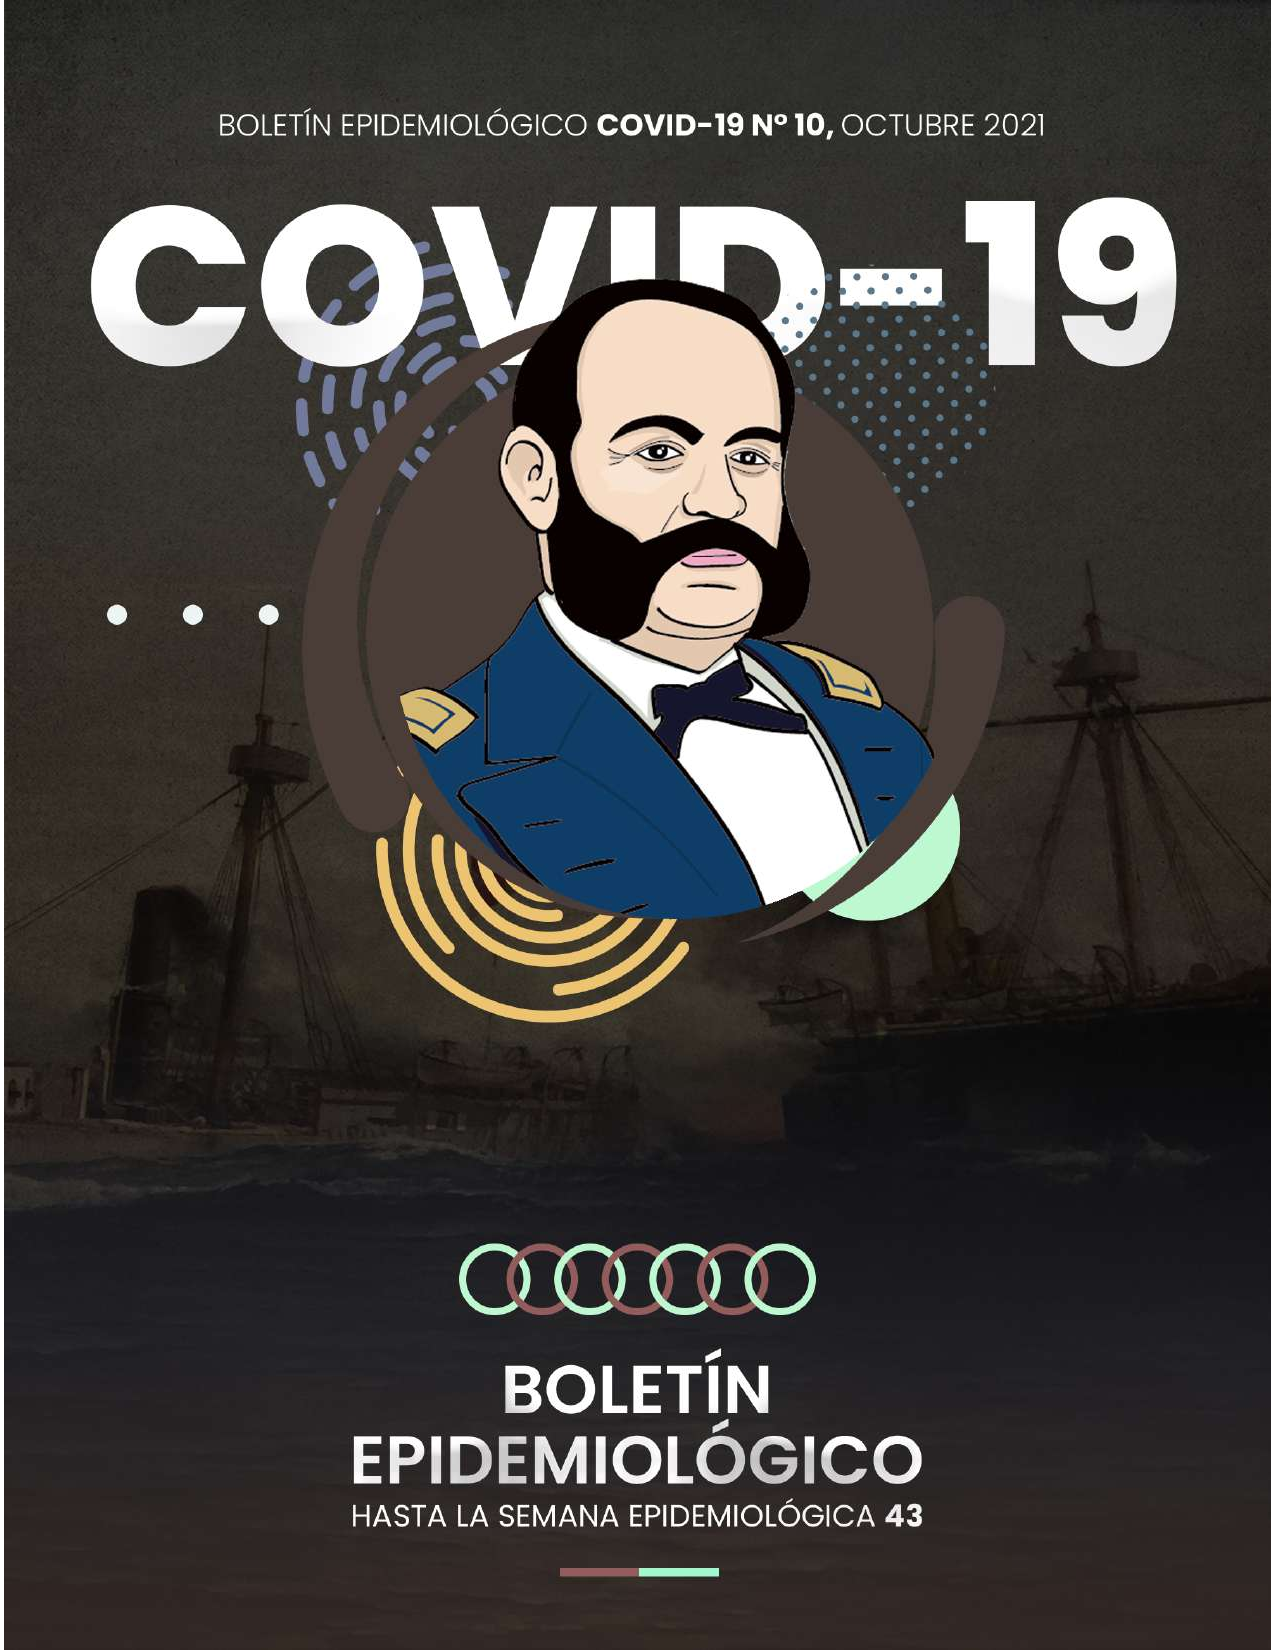
\includepdf[pages={1}]{../editorial/portada.pdf}
	\clearpage
	
	\pagestyle{plain}\pagenumbering{arabic}
	
	\clearpage
	
	
	\begin{center}
	
		{\large Gerencia Regional de Salud}
		
		\textbf{MSP. Javier Ramírez Escóbar}
		
		Gerente Regional \vspace{1.0cm}
		
		Dirección Ejecutiva de Inteligencia Sanitaria
		
		\textbf{MSP. Darío Francisco Navarro Mendoza}
		
		Director
		
		\vspace{1.5cm}
\noindent
\begin{minipage}[t]{.45\textwidth}
	\centering
	Dirección de Epidemiología e Investigación  \\
	\textbf{MSC. Fátima R. Concha Velasco}\\
	Directora \vspace{1.0cm}\\
	% Por orden alfabético del apellido
	\textit{Equipo de Epidemiología e Investigación }\vspace{.5cm}\\
	Econ. Karen Yorka Aguilar Zuñiga \\
	M.C Edwards Adrian Aguirre Valenzuela \\
	Lic. Nadia Isabel Cáceres Pillco \\
	TAP. Edgar Waldo Capcha Salcedo \\
	M.S.P. Pablo Fidel Grajeda Ancca \\
	M.C. Katia Luque Quispe \\
	M.C. Ana Gabriela Eulalia Moncada Arias \\
	Lic. Enf. Ruth Nelly Oscco Abarca \\
	Ing. Joel Wilfredo Sumerente Ayerbe \\
	Lic. Enf. Guinetta Margarita Yabar Herrera \vspace{1.5cm}\\	
\end{minipage}
\hfill
\noindent
\begin{minipage}[t]{.45\textwidth}
	\centering
	Dirección de Estadística, Informática y Telecomunicaciones\\
	\textbf{Ing. Abel Rimasca Chacón} \\
	Director \vspace{1.0cm} \\
	% Por orden alfabético del apellido
	\textit{Equipo de Estadística, Informática y Telecomunicaciones} \vspace{.5cm} \\
	Ing. Iván Atayupanqui Rondón \\
	Ing. Miguel Ángel Campana Alarcón \\
	Ing. Uriel Lacuta Farfán \\
	Ing. Jorge Fernando Lovatón Ramos \\
	Ing. Danny Robert Moscoso Sánchez \\
	Lic. Ray Milton Valderrama Álverez \vspace{1.5cm}\\
\end{minipage}
Secretaria: Sra. Ruth Baca Mendoza
	\end{center}
\let\cleardoublepage\clearpage
	\tableofcontents
	
	%\mainmatter
	%---------------------------------------------------------------------------
	% CAPÍTULO: EDITORIAL
	%---------------------------------------------------------------------------

	\pagebreak
	
	\section*{Editorial}	\addcontentsline{toc}{chapter}{Editorial}
	\begin{wrapfigure}{l}{8.5cm}
		\label{wrap-fig:1}
		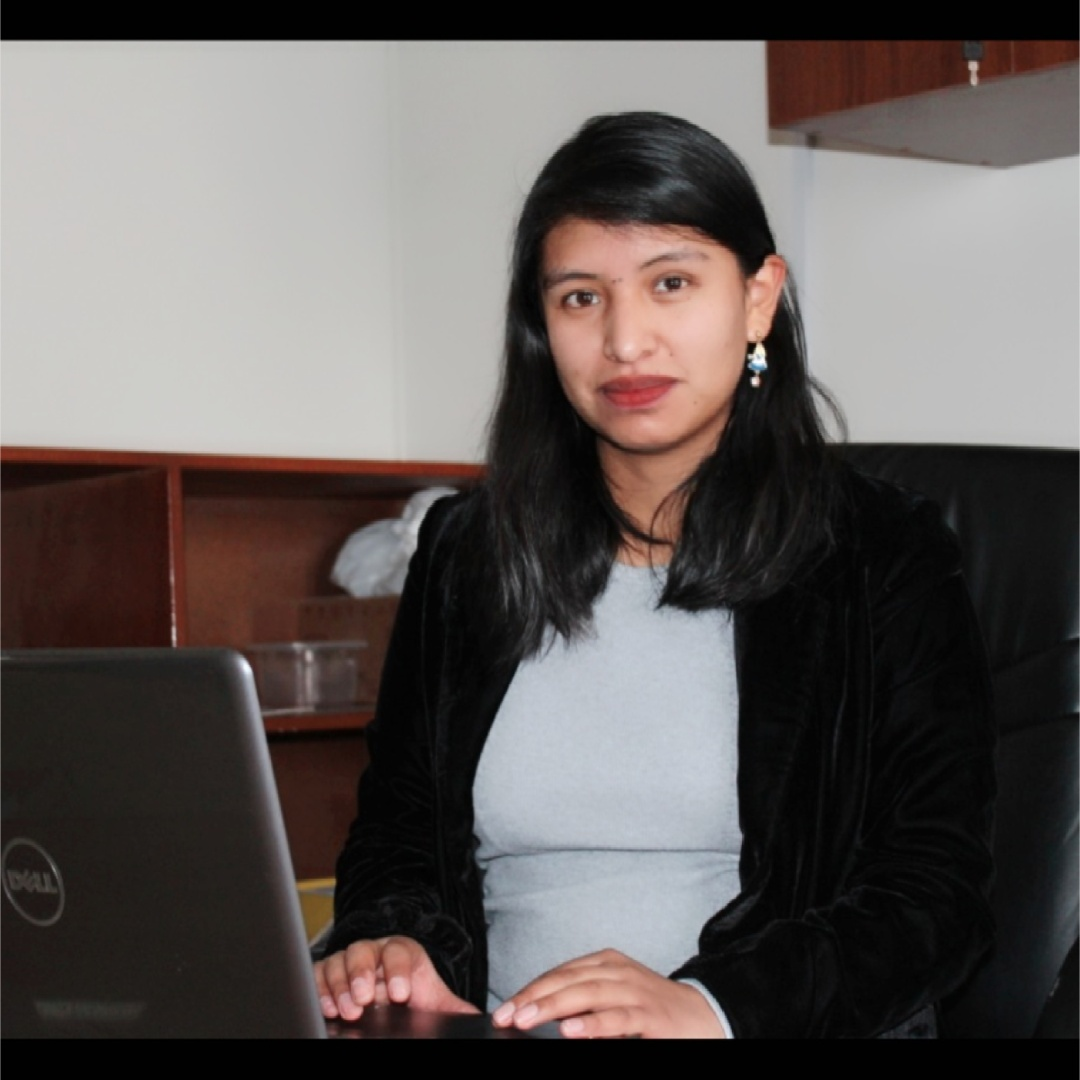
\includegraphics[width=8.5cm]{../editorial/foto_ana_editorial}
		\caption*{
			\centering
				MC. Ana Gabriela Moncada Arias
				
				\textit{Dirección de Epidemiología e Investigación}
				
				GERESA, Cusco }
	\end{wrapfigure}
	
	\noindent Hace más de un año desde que el SARS-CoV2 (causante de la Enfermedad por COVID-19) apareció en nuestras vidas para dar lugar a la pandemia del siglo XXI. Su expansión rápida llevo a los límites a diversos sistemas de salud de todo el mundo y generó la muerte de miles de personas.  Pero junto al principio de la pandemia, también se daría lugar al inicio de otra epidemia: la desinformación. A pesar de que la desinformación  ha estado presente por mucho tiempo en nuestras vidas, la pandemia la exacerbó a su máximo nivel. 
	
	Y es que los recursos tecnológicos actuales permite la transmisión de información a velocidades nunca antes vistas, y en diversos formatos incluyendo los audiovisuales. La creación de contenido informativo no solo está restringido a personas conocedoras del tema, sino también a personas que dinfunden información que solo beneficia intereses personales . Estos factores generan un nicho perfecto como para que contenido de dudosa calidad pero llamativos para el ciudadano de a pie se difundan fácilmente. 
	
	El miedo a las vacunas suele ser infundido por información incorrecta que no es verificada por la población, y que aunado a un desconocimiento y al  miedo a los cambios y a lo nuevo, terminan en una actitud que reta los grandes avances que se realizan en salud pública.
	
	Uno de los ejemplos más concretos que podemos encontrar es el del movimiento antivacunas. Este movimiento inicia junto al inicio del proceso de vacunación durante el siglo XIX, y que tomo mayor énfasis durante el siglo XX debido a la publicación de un estudio que relacionaba el transtorno de espectro autista y otras enfermedades con las vacunas. Actualmente, nuevos estudios han demostrado que las vacunas son seguras, y no generan mayores efectos adversos a largo plazo.  Las vacunas salvan vidas y no hay dudas. En ellas se depositó la esperanza para vencer al SARS-CoV-2. Pero, aun con todas las vidas que se perdieron durante la pandemia, el sufrimiento vivido  y  con vacunas disponibles, existe un porcentaje no despreciable de la población mundial y local que no desea vacunarse. 
	
	
	En nuestra comunidad local, este riesgo es aún mayor debido a la poca alfabetización sanitaria que posee la población general. Pero como cualquier reto en salud pública, este debe ser afrontado de manera conjunta por todos los actores: ciudadanía, autoridades y organizaciones. Solo la información adecuada, dada de forma correcta por todos el sistema sanitario podrá combatir la epidemia de desinformación que solo prolonga el final de esta pandemia. El mensaje debe transmitirse, las vacunas salvan vidas y la mejor vacuna es la que llega primero.
	
	%---------------------------------------------------------------------------
	% CAPÍTULO: METODOLOGÍA
	%---------------------------------------------------------------------------
			%insertar el cover del capitulo
	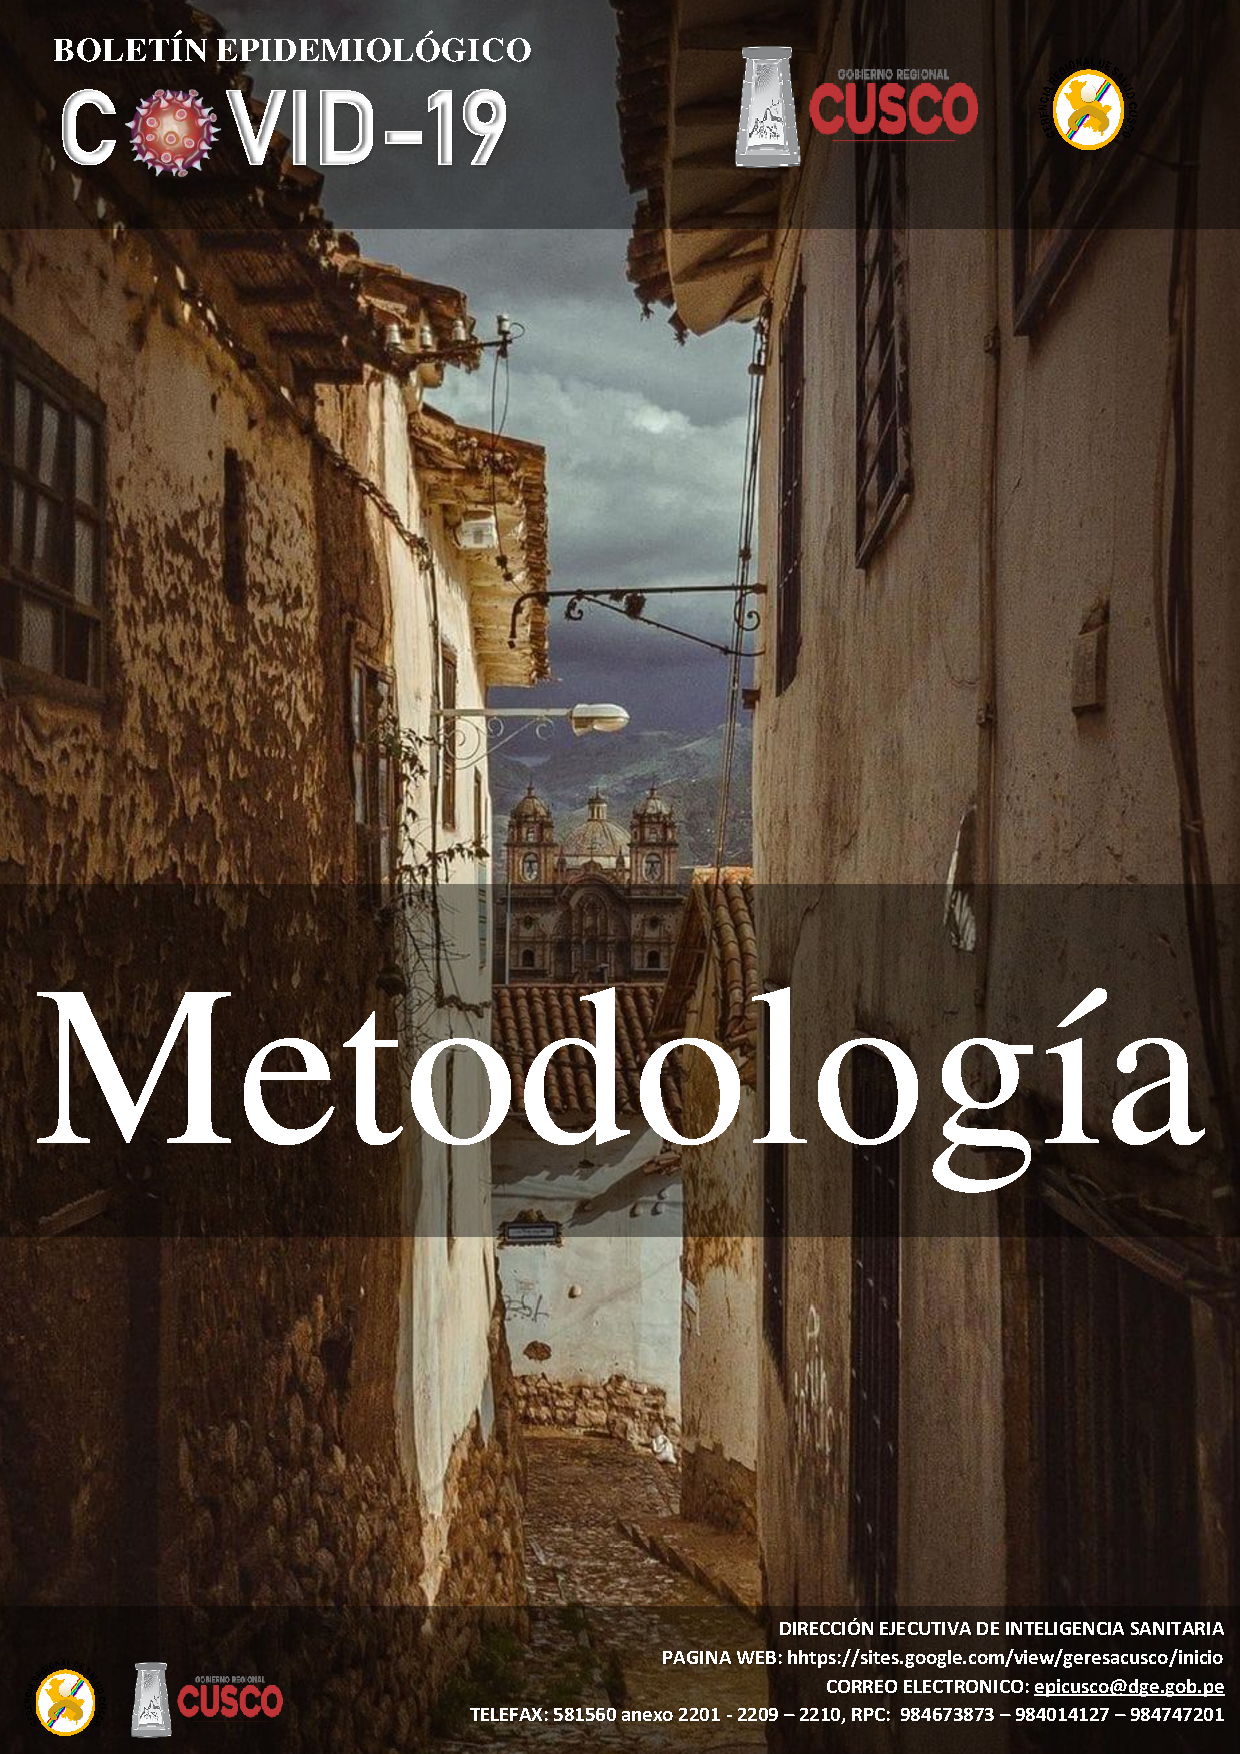
\includepdf[pages={1}]{../editorial/1.pdf}
	\clearpage
	
	\section*{Metodología}	
	\addcontentsline{toc}{chapter}{Metodología}
	Se describe la metodologia 
	\noindent El presente Boletín tiene el objetivo de informar sobre los principales indicadores epidemiológicos y de gestión hospitalaria,  para hacer el seguimiento de la pandemia en nuestra región y tomar mejores decisiones. Este Boletín tiene una metodología de tipo descriptiva. 
	
	En él, se encuentra un análisis extensivo de la situación actual de la pandemia en nuestra región desde la semana epidemiológica (SE) 1 a la 47 del 2021 (3 de enero al 28 de noviembre del 2021).
	
	Los datos analizados incluyeron: a) características generales: sexo, edad, casos confirmados, fallecidos; b) características clínicas: síntomas reportados, casos confirmados sintomáticos, casos confirmados asintomáticos y comorbilidades; c) indicadores epidemiológicos: sistema de vigilancia epidemiológica, tasa de mortalidad, tasa de positividad de pruebas diagnósticas, casos activos – recuperados, y exceso de muerte por todas las causas, y d) indicadores de gestión hospitalaria: , ocupación de camas UCI y No.UCI en la Región.
	
	Las fuentes de información son las bases de datos de NOTI WEB (aplicativo del Sistema de Vigilancia Epidemiológica - COVID-19), SISCOVID (Sistema Integrado para COVID-19), SINADEF (Sistema Informático Nacional de Defunciones), SICOVAC-HIS MINSA(Base de datos de vacunación por COVID-19), Reporte de Disponibilidad de Camas de Hospitalización y datos de la Oficina de Referencias-Contrarreferencias de la Dirección de Emergencias y Desastres de GERESA-Cusco. 
	
	Se usaron frecuencias absolutas y relativas para la descripción de los datos cualitativos. Para la descripción de datos cuantitativos se calcularon tasas (mortalidad, pruebas diagnósticas, incidencia de casos), promedios (ocupación de camas hospitalarias, fallecidos por COVID y fallecidos por todas las causas). Para describir la tendencia se representaron los datos cuantitativos y frecuencias relativas en intervalos de 7 días (semana epidemiológica). En las variables de sistema de vigilancia epidemiológica (1 prueba por 100,000 habitantes) y ocupación de cama (adecuado, menor a $70\%$, moderado, entre $75$ a $90\%$ y limitado, más de $90\%$), siendo todos los puntos de referencia sugeridos por la Organización Mundial de la Salud. Para el análisis de exceso de mortalidad, se usó la metodología descrita por C. Giattino, H. Ritchie, M. Roser, E. Ortiz-Ospina, y J. Hasell en el artículo ``Excess mortality during the Coronavirus pandemic (COVID-19)''. Published online at OurWorldInData.org.
	
	La descripción de dichas variables se hace de manera regional y provincial. En la presente edición se hace una descripción de la tasa de incidencia, tasa de mortalidad, tasa de positividad por prueba molecular y antigénica, y exceso de defunciones de todas las provincias de nuestra región. El lector interesado en un análisis distrital de los casos y defunciones puede encontrar en los links correspondientes.
	 
	%---------------------------------------------------------------------------
	% CAPÍTULO: CARACTERÍSTICAS GENERALES
	%---------------------------------------------------------------------------
		%insertar el cover del capitulo
	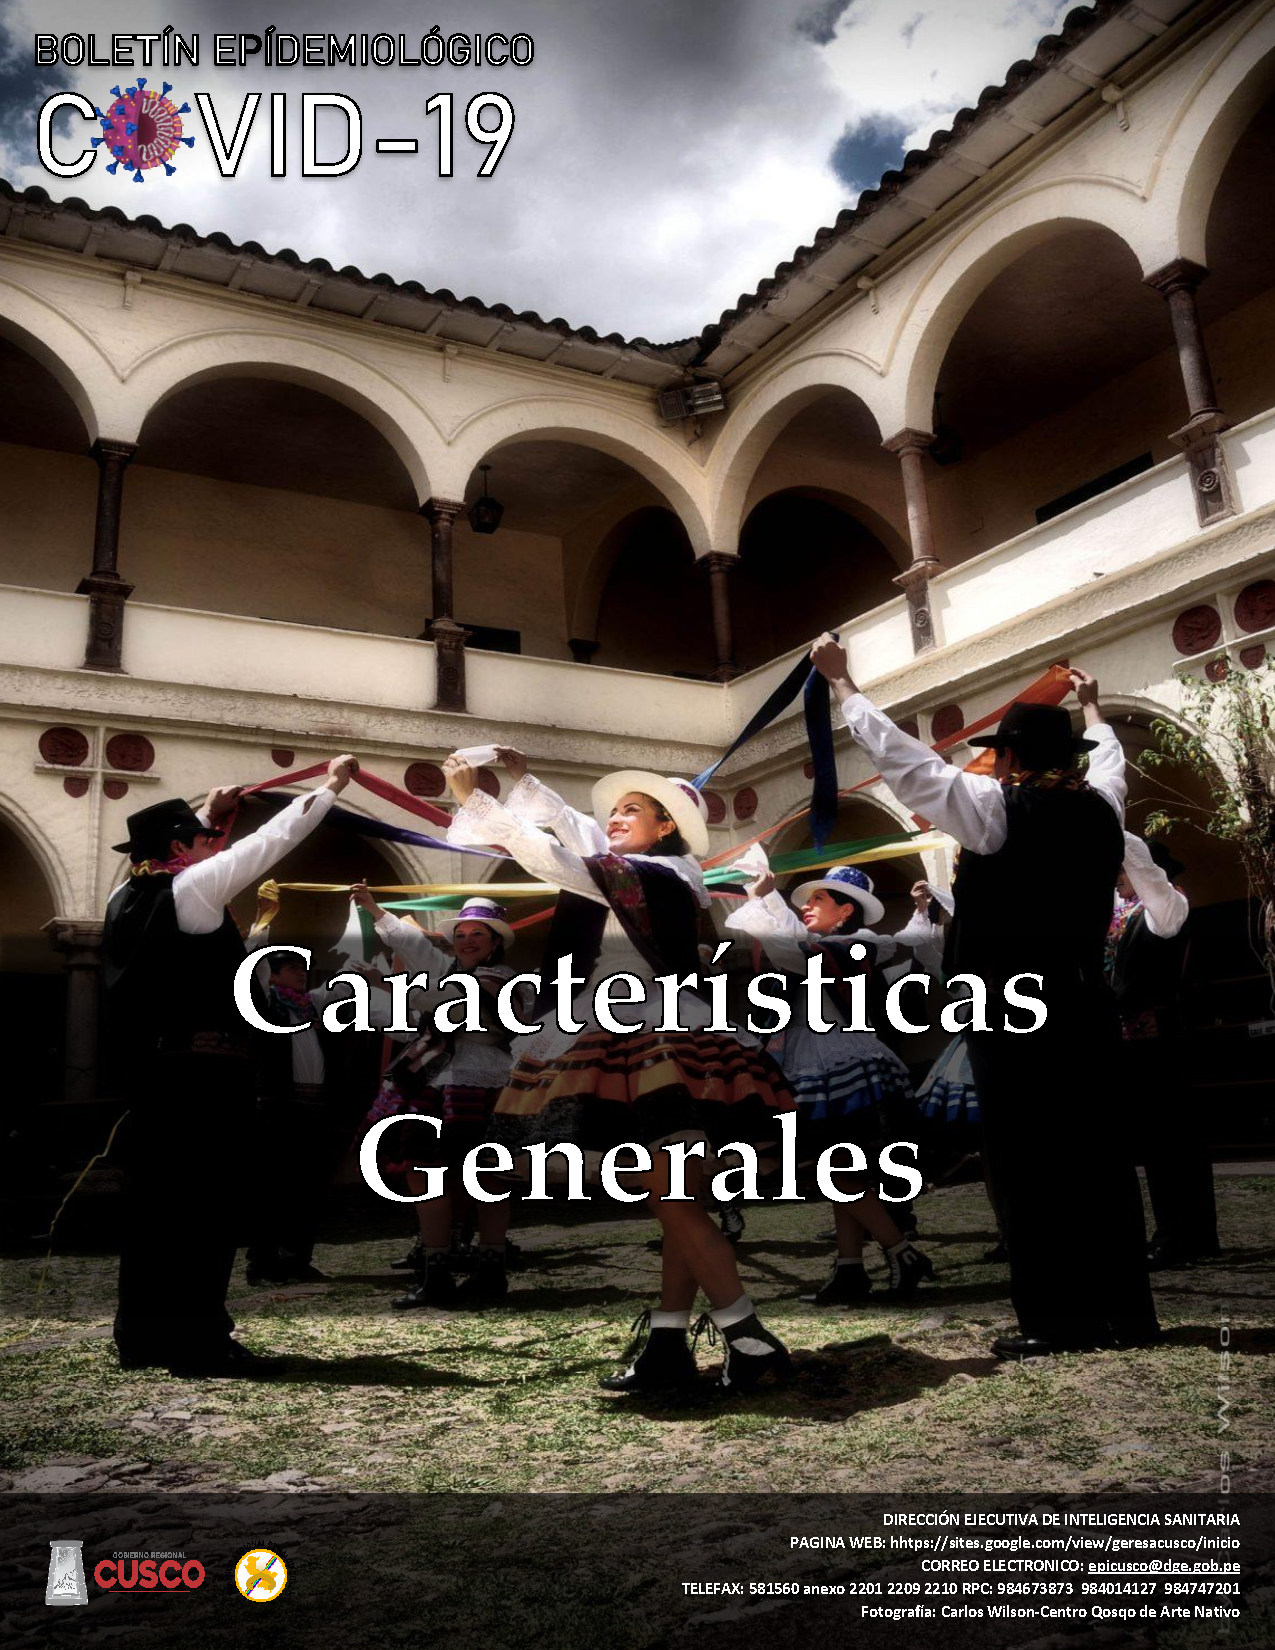
\includepdf[pages={1}]{../editorial/2.pdf}
	\clearpage	
	\section*{Características Generales}
	\addcontentsline{toc}{chapter}{Características Generales}
	
	
	
 	\noindent En la Figura \ref{fig:casos_edad_sexo} muestra la cantidad de casos confirmados de COVID-19 hasta la SE 43 por grupo etario (en intervalos de 10 años) y sexo. La mayor cantidad de casos se concentra en los grupos etarios de 30 a 39 años, con un total de 17 546 casos acumulados, seguido del grupo etario de 20 a 29 años, con un total de 16 022. Es preciso recalcar que en los grupos etarios de 30 hasta 59 años, el sexo masculino es el más afectado por COVID-19, en el resto de grupos etarios el sexo más afectado es el femenino. 
 	
 	
 	
	\begin{figure}[h]
		\caption{Casos Confirmados de COVID-19 según Grupo de Edad y Sexo en la Región Cusco, hasta la SE 43.}\label{fig:casos_edad_sexo}
		\begin{center}
			\includegraphics[width=0.65\linewidth]{../figuras/1_casos.pdf}
		\end{center}
		{\footnotesize {Fuente de datos: SISCOVID, NOTICOVID.}}
	\end{figure}
\pagebreak

La Figura  \ref{fig:fallecidos_edad_sexo}  muestra el número de muertes debido a COVID-19 por grupo etario y sexo. Se puede apreciar que el mayor número de muertes se reporta en el grupo etario de 70 a 79 años(772 muertes acumuladas), seguido del grupo etario de 60 a 69 años (709 muertes acumuladas). Cabe mencionar que en casi todos los grupos etarios la cantidad de fallecidos correspondientes al sexo masculino supera a la cantidad de fallecidos de sexo femenino.
	\begin{figure}[h]
		\caption{Casos fallecidos por COVID-19 según Grupo de Edad y Sexo en la Región Cusco, hasta la SE 43, 2021}\label{fig:fallecidos_edad_sexo}
		\begin{center}
			\includegraphics[width=0.65\linewidth]{../figuras/2_muertes.pdf}
		\end{center}
		{\footnotesize {Fuente de datos: SISCOVID, NOTICOVID.}}
	\end{figure}


\cleardoublepage
%---------------------------------------------------------------------------
% CAPÍTULO: CARACTERÍSTICAS CLÍNICAS
%---------------------------------------------------------------------------
	%insertar el cover del capitulo
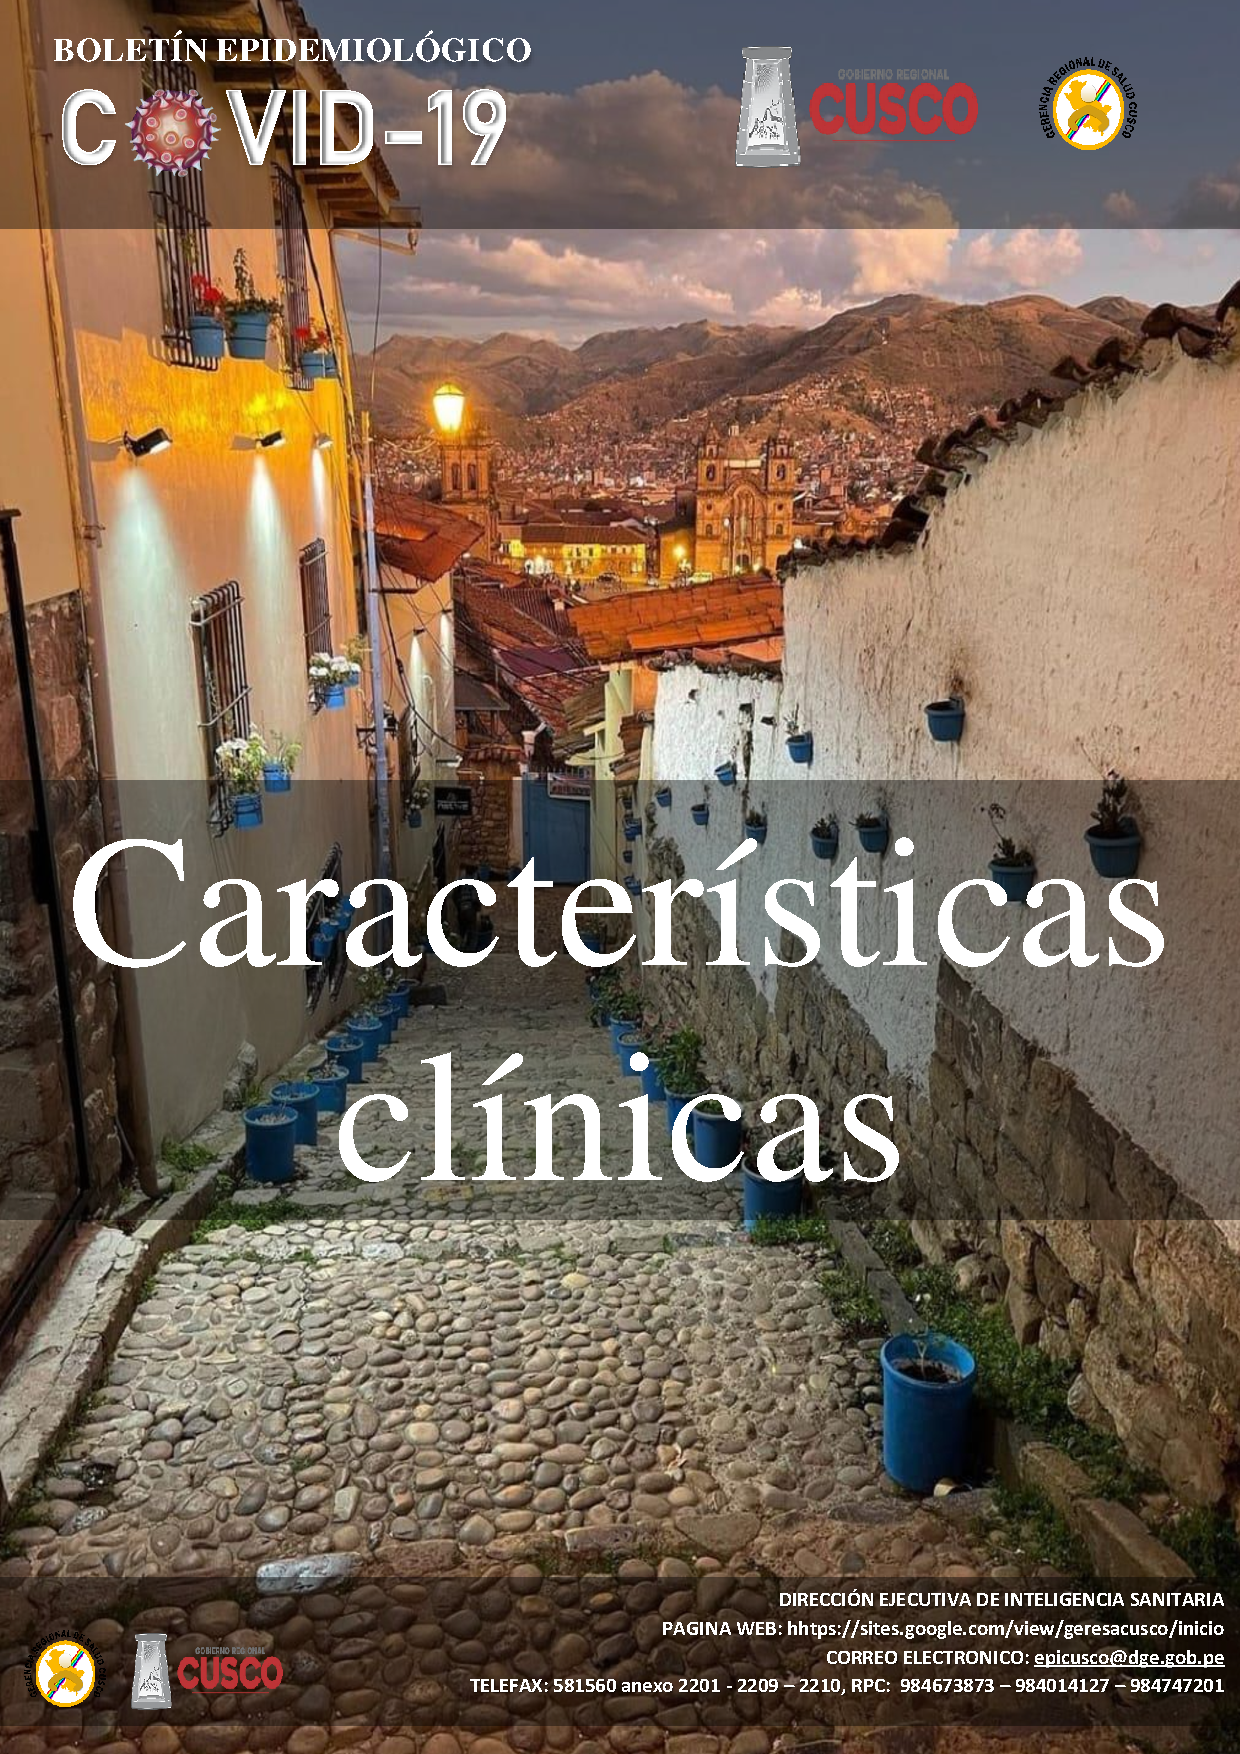
\includepdf[pages={1}]{../editorial/3.pdf}

\clearpage

\section*{Características Clínicas}
\addcontentsline{toc}{chapter}{Características Clínicas}	


\noindent En la Figura \ref{fig:sintomas}, se presentan los síntomas más frecuentes de los pacientes diagnosticados con COVID-19, el síntomas más frecuente es la tos (15$\%$), seguido de dolor de garganta (14,3$\%$). Con respecto a los signos clínicos, en la Figura \ref{fig:signos} se evidencia que el exudado faríngeo (63,8$\%$) es el signo más frecuente. 

\begin{figure}[h]
	\caption{Síntomas más frecuentes de los pacientes diagnosticados por COVID-19 en la Región Cusco, hasta la SE 47, 2020-2021.  }\label{fig:sintomas}
	\begin{center}
		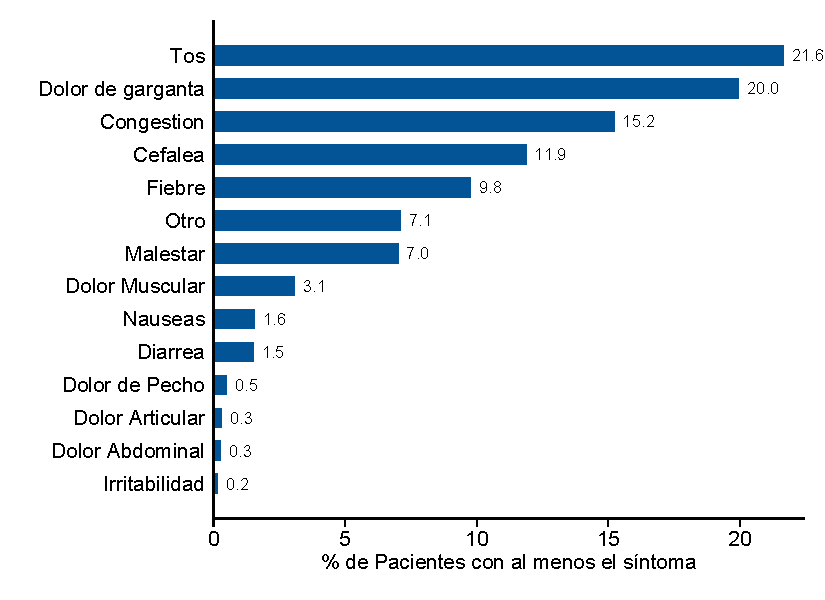
\includegraphics[width=0.85\linewidth]{../figuras/figura_sintoma.pdf}
	\end{center}
	{\footnotesize {Fuente de datos: SISCOVID, NOTICOVID.}}
\end{figure}

\begin{figure}[h]
	\caption{Signos más frecuentes de los pacientes diagnosticados por COVID-19 en la Región Cusco, hasta la SE 47, 2021.}\label{fig:signos}
	\begin{center}
		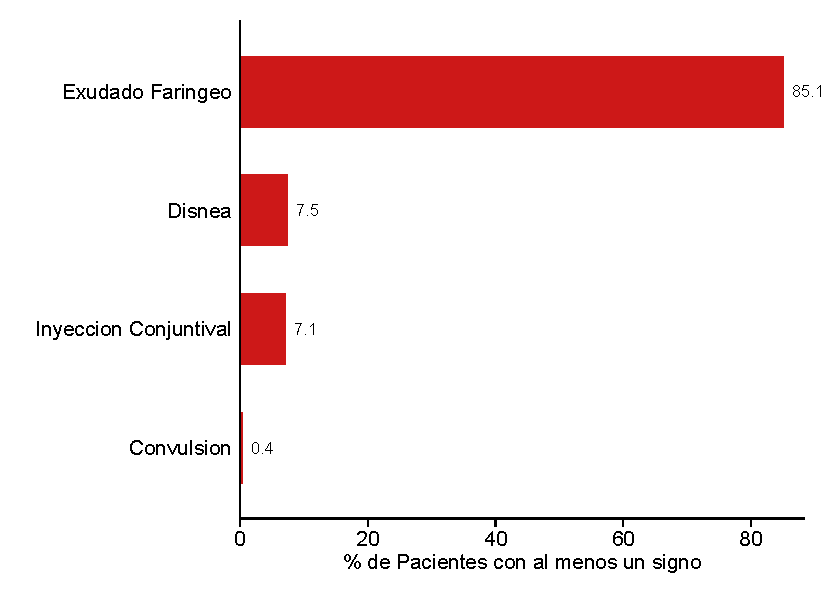
\includegraphics[width=0.65\linewidth]{../figuras/figura_signo.pdf}
	\end{center}
	{\footnotesize {Fuente de datos: NOTICOVID.}}
\end{figure}

La comorbilidades más frecuentes se encuentran graficadas en la Figura \ref{fig:comorbilidades}. La obesidad es la comorbilidad más frecuente con una prevalencia de 26,5$\%$, seguido de Diabetes con 22,2$\%$. 

\begin{figure}[h]
	\caption{Comorbilidades más frecuentes de los pacientes diagnosticados por COVID-19 en la Región Cusco, hasta la SE 47, 2021. }\label{fig:comorbilidades}
	\begin{center}
		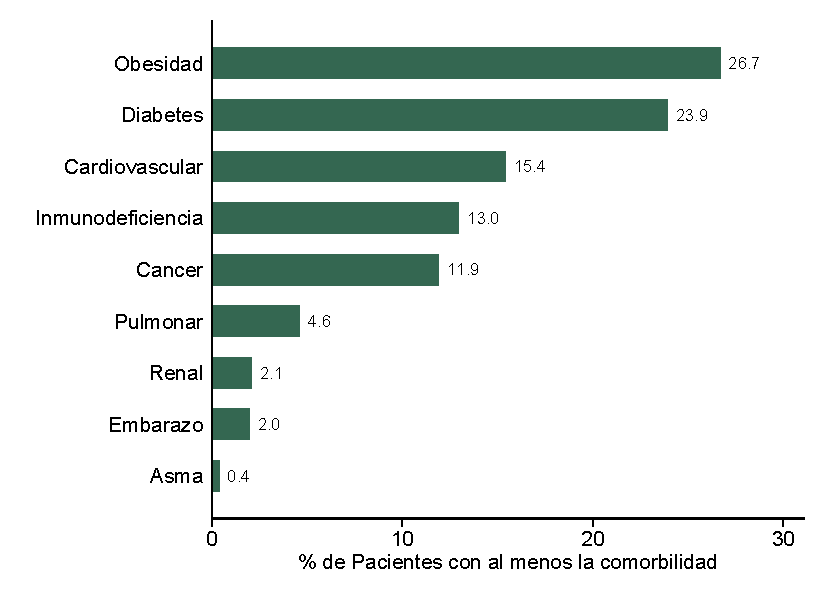
\includegraphics[width=0.65\linewidth]{../figuras/figura_comorbilidad.pdf}
	\end{center}
	{\footnotesize {Fuente de datos: NOTICOVID.}}
\end{figure}
\clearpage
 En la Figura \ref{fig:sintomaticos_asintomati} se evidencia la curva epidémica de casos sintomáticos y asintomáticos durante toda la pandemia, comparada con los casos sintomáticos y asintomáticos del 2020. Se evidencia que hubo un incremento discreto de casos asintomáticos en la SE 43 y su posterior descenso para la SE 46. Con respecto a los casos sintomáticos, la tendencia fue constante desde la SE 29.  
 
 
\begin{figure}[h]
	\caption{Casos Sintomáticos y Asintomáticos de COVID-19, por Semana Epidemiológica en la Región Cusco, hasta la SE 47,2021.  }\label{fig:sintomaticos_asintomati}
	
	\begin{center}
		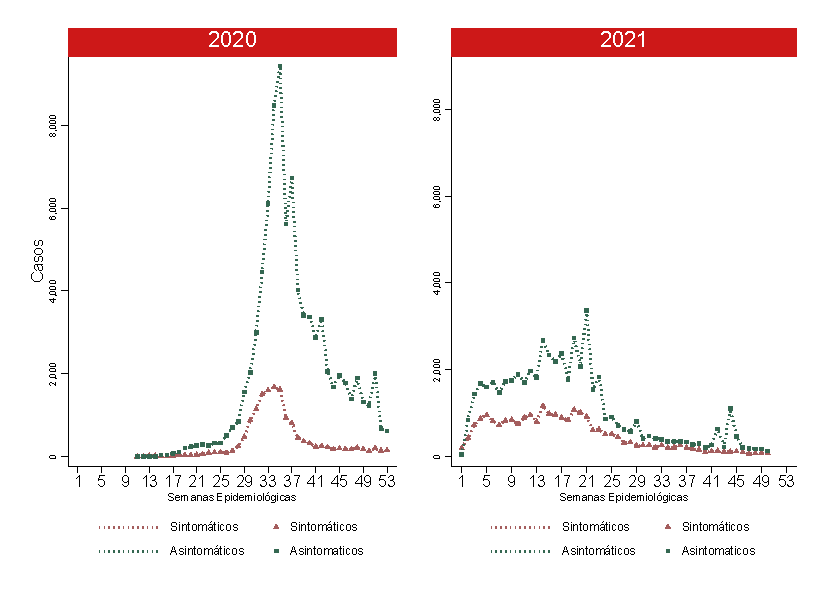
\includegraphics[width=0.75\linewidth]{../figuras/sintomaticos_20_21.pdf}
	\end{center}
	{\footnotesize {Fuente de datos: SISCOVID, NOTICOVID.}}
\end{figure}
\clearpage

%---------------------------------------------------------------------------
% CAPÍTULO: ANÁLISIS DE INDICADORES
%---------------------------------------------------------------------------
%insertar el cover del capitulo
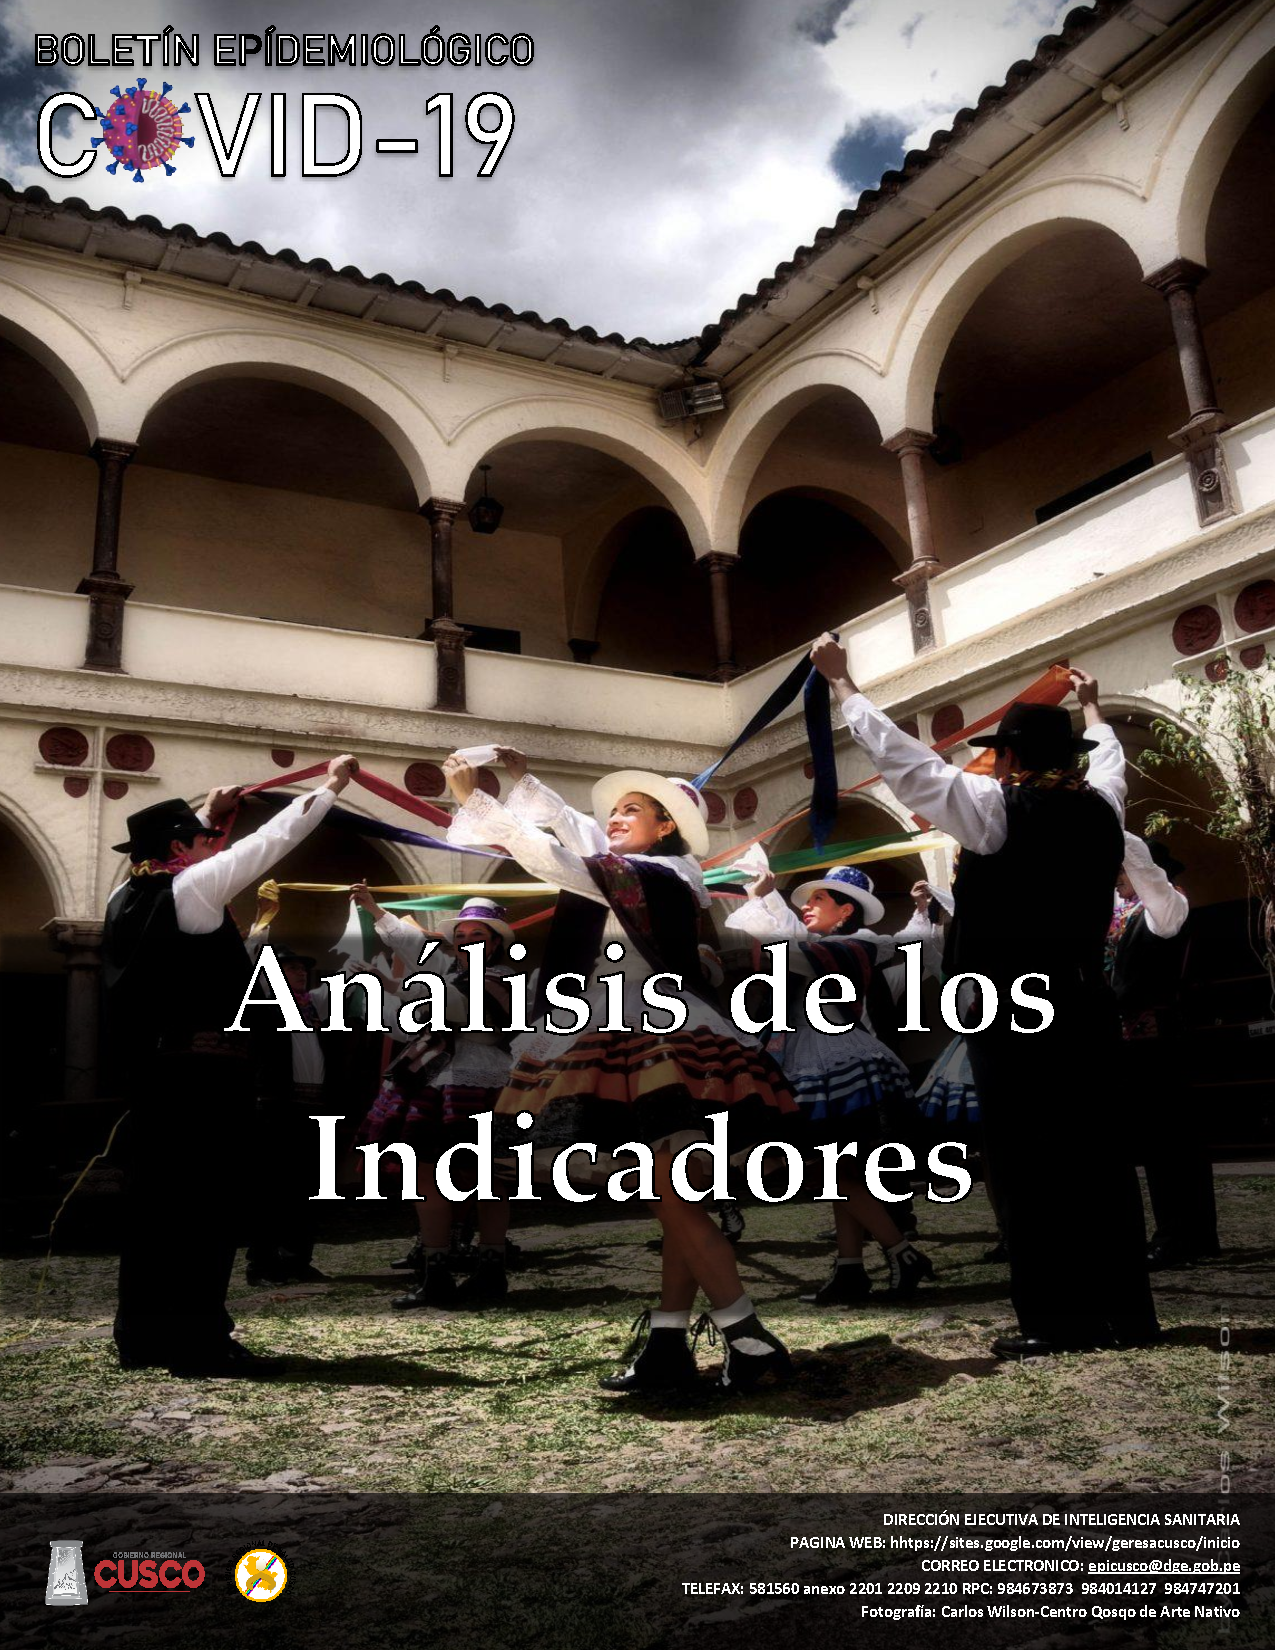
\includepdf[pages={1}]{../editorial/4.pdf}
\clearpage

    \section*{Análisis de Indicadores}
    \addcontentsline{toc}{chapter}{Análisis de Indicadores}
   	\subsection*{Tasa de Incidencia y Tasa de Positividad}
\noindent La evolución de la Tasa de Incidencia en el tiempo se encuentra graficada en la Figura \ref{fig:incidencia}, se observa que hubo una tendencia a la disminución hasta la SE 41 (23 casos/100 000 * personas) tras lo cuál la pendiente de casos nuevos va en ascenso, llegando a registrarse una tasa de incidencia de 57 casos/100 000* personas, el número más alto registrado desde la SE 31.

   \begin{figure}[h]
   	\caption{Tasa de Incidencia de COVID-19 en la región Cusco hasta la SE 43. }\label{fig:incidencia}
   	\begin{center}
   		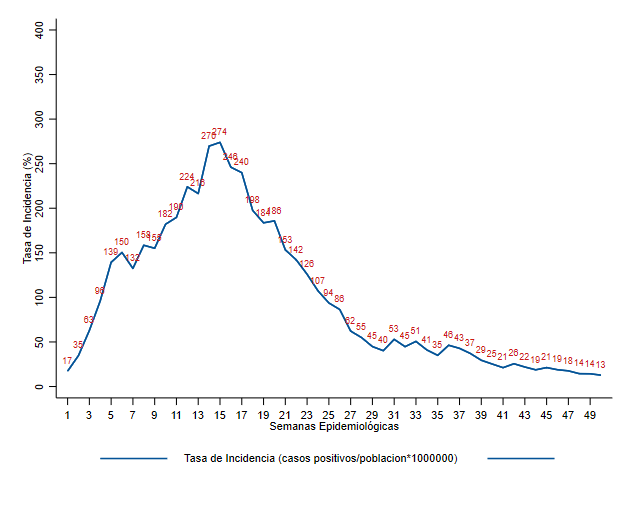
\includegraphics[width=0.65\linewidth]{../figuras/tasa_incidencia}
   	\end{center}
   	{\footnotesize {Fuente de datos: SISCOVID, NOTICOVID.}}
   \end{figure}
   
   La Figura \ref{fig:total_muestras_procesada} muestra un comparativo de las Tasas de Positividad ($\%$) de pruebas moleculares y antigénicas. Se observa que desde la SE 27, la tasa de positividad de pruebas antigénicas tuvo una pendiente en descenso, llegando a reportar el porcentaje mas bajo durante todo el año durante la SE 43 (4 $\%$ de pruebas positivas). 
   
  
   
   \begin{figure}[h]
   	\caption{Tasa de positividad para muestras antigénicas y moleculares por COVID-19 en la región Cusco hasta la SE 43. }\label{fig:total_muestras_procesada}
   	\begin{center}
   		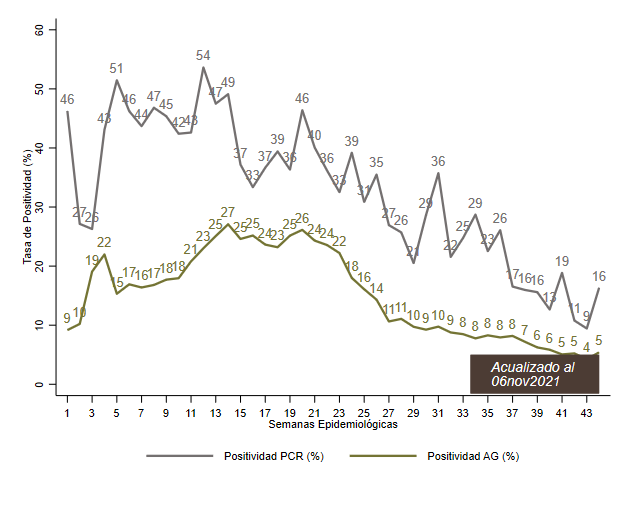
\includegraphics[width=0.65\linewidth]{../figuras/positividad_diaria.pdf}
   	\end{center}
   	{\footnotesize {Fuente de datos: SISCOVID, NOTICOVID.}}
   \end{figure}



La Figura \ref{fig:positividad_ambas} muestra el comparativo de las tasas de positividad y el número de pruebas positivas antigénicas y moleculares. Con respecto a las pruebas moleculares, la tasa de positividad ha sido variable a lo largo de las cuatro últimas semanas presentando una pendiente en descenso en las últimas 2 semanas,al igual que la tasa de positividad de pruebas antigénicas que ha descendido discretamente desde la SE 44.  

\begin{landscape}
   \begin{figure}[h]
	\caption{Positividad y Tasa de Positividad de muestras moleculares y antigénicas tomadas por COVID-19 en la región Cusco, hasta la SE 47. }\label{fig:positividad_ambas}
   	\begin{center}
   		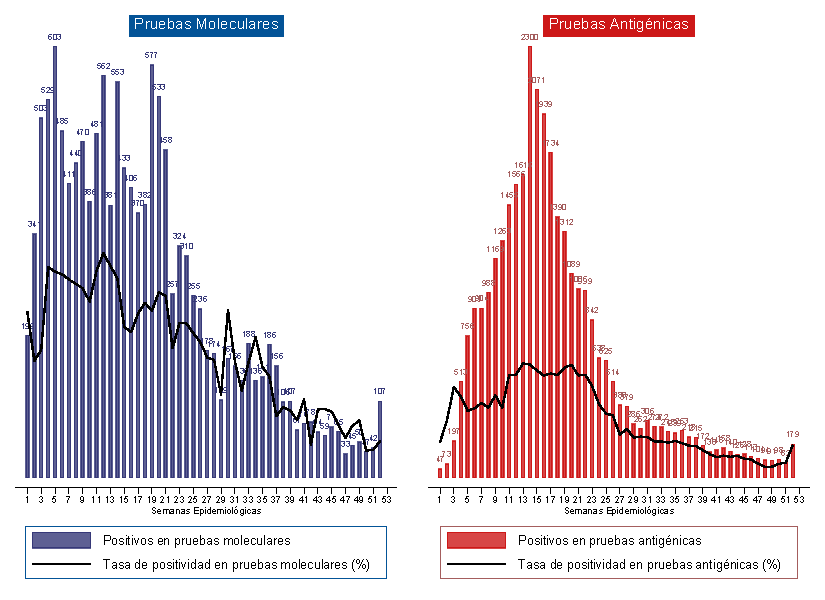
\includegraphics[width=0.85\linewidth]{../figuras/positividad_ambas.pdf}
   	\end{center}
   	{\footnotesize {Fuente de datos: SISCOVID, NOTICOVID.}}
   \end{figure}
\end{landscape}
\clearpage

	\subsection*{Análisis de la Mortalidad}

	\noindent En la Figura \ref{fig:mortalidad_edad} muestra la mortalidad semanal para las edades agrupadas en diez años. Se evidencia que la tasa de mortalidad más alta se encuentra en el grupo etario de 80 años a más, presentando un pico de muertes para la SE 46. En segundo lugar se encuentra el grupo etario de 70 a 79 años, cuya tasa de mortalidad presentó un discreto incremento para la SE 45, tras la cuál presenta una tendencia al descenso. La tasa de mortalidad en el resto de grupos etarios se ha mantenido baja.
	
	\begin{figure}[h]
	\caption{Tasa de Mortalidad por COVID-19 por Grupos Etarios, hasta la SE 47, 2021.}\label{fig:mortalidad_edad}
	\begin{center}
		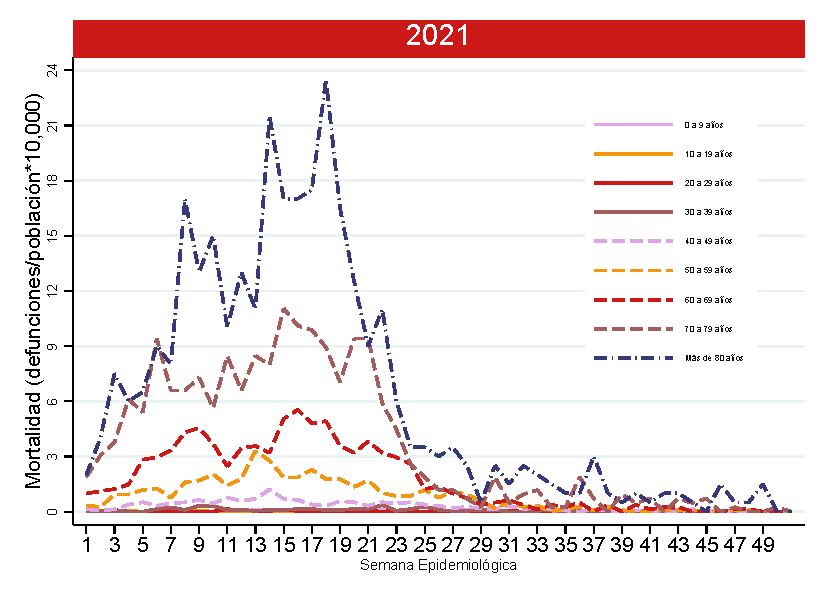
\includegraphics[width=0.65\linewidth]{../figuras/mortalidad_edad.pdf}
	\end{center}
	{\footnotesize Fuente de datos: SINADEF} 
	\end{figure}


	La Figura \ref{fig:mortalidad_grupo_edad} muestra la relación entre la tasa de mortalidad y la vacunación. Las líneas de referencia representan las fechas del inicio de la vacunación (primera y segunda dosis) para el correspondiente grupo etario. 
	
	Se observa que tras la administración de dos dosis de vacuna contra COVID-19,  hay una pendiente marcada en descenso de la tasa de mortalidad, excepto en el grupo etario de 30 a 39 años, cuya tasa de mortalidad ha sido baja desde antes de la vacunación.

	\begin{figure}[h]
	\caption{Tasa de Mortalidad por COVID-19 por Grupos Etarios, hasta la SE 47, 2021.}
	\label{fig:mortalidad_grupo_edad}
	\centering
	\begin{subfigure}[b]{0.45\textwidth}
		\centering
		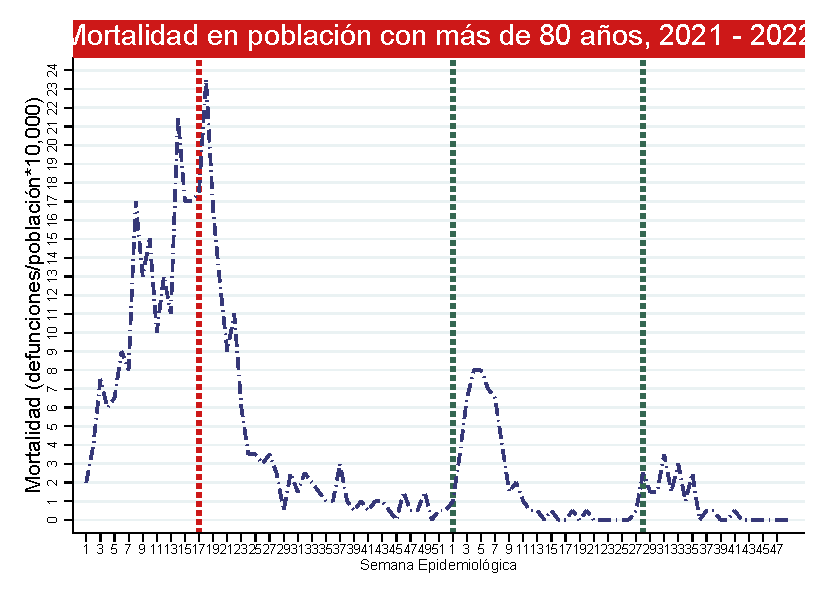
\includegraphics[width=\textwidth]{../figuras/mortalidad_edad_80.pdf}
		\caption{Más de 80 años}
		%\label{fig:}
	\end{subfigure}
	\hfill
	\begin{subfigure}[b]{0.45\textwidth}
		\centering
		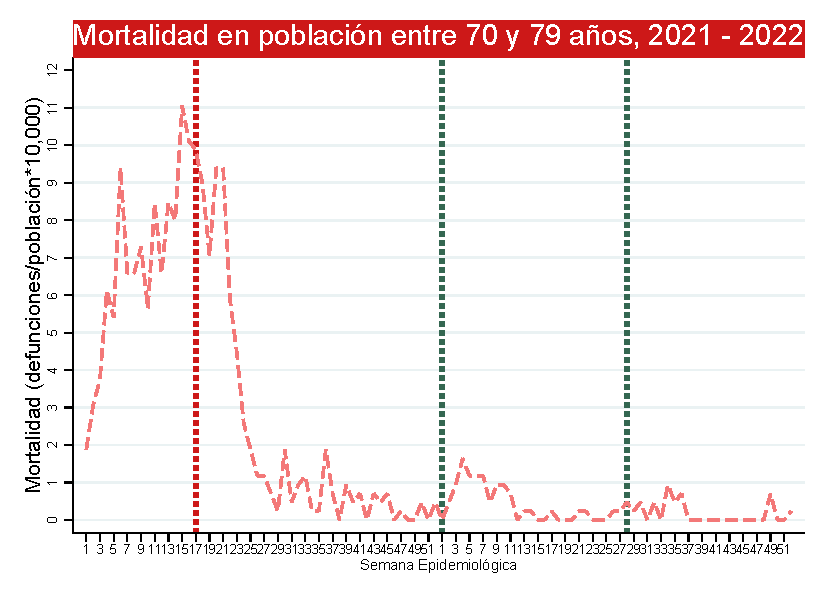
\includegraphics[width=\textwidth]{../figuras/mortalidad_edad_70.pdf}
		\caption{70 a 79 años}
		%\label{fig:70 a 79 años}
	\end{subfigure}

	\vspace{10mm}
	\begin{subfigure}[b]{0.45\textwidth}
		\centering
		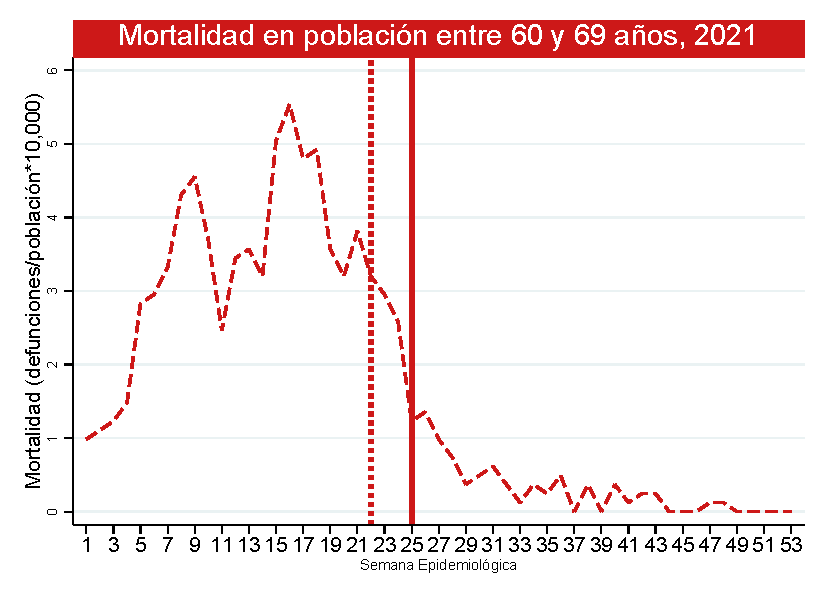
\includegraphics[width=\textwidth]{../figuras/mortalidad_edad_60.pdf}
		\caption{60 a 69 años}
		%\label{fig:60 a 69 años}
	\end{subfigure}
	\hfill
	\begin{subfigure}[b]{0.45\textwidth}
		\centering
		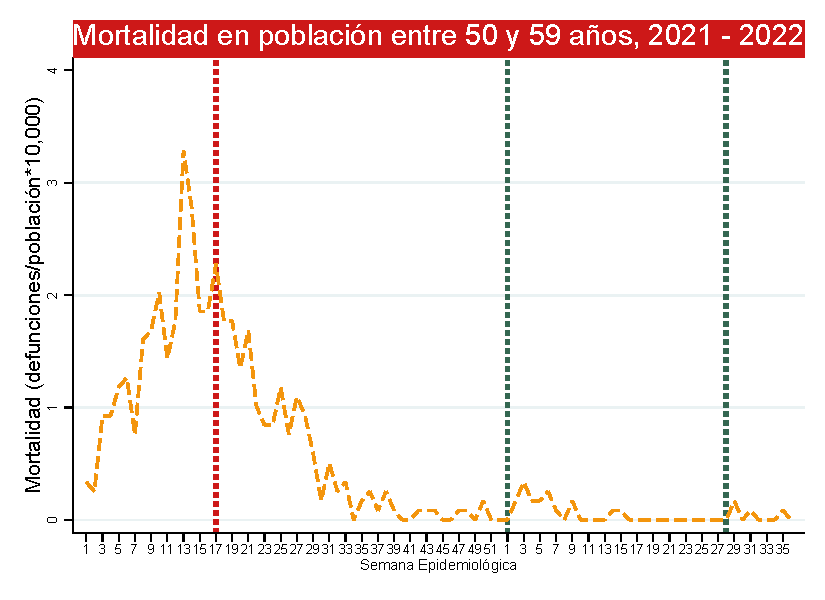
\includegraphics[width=\textwidth]{../figuras/mortalidad_edad_50.pdf}
		\caption{50 a 59 años}
		%\label{fig:50 a 59 años}
	\end{subfigure}

	\vspace{10mm}
	\begin{subfigure}[b]{0.45\textwidth}
		\centering
		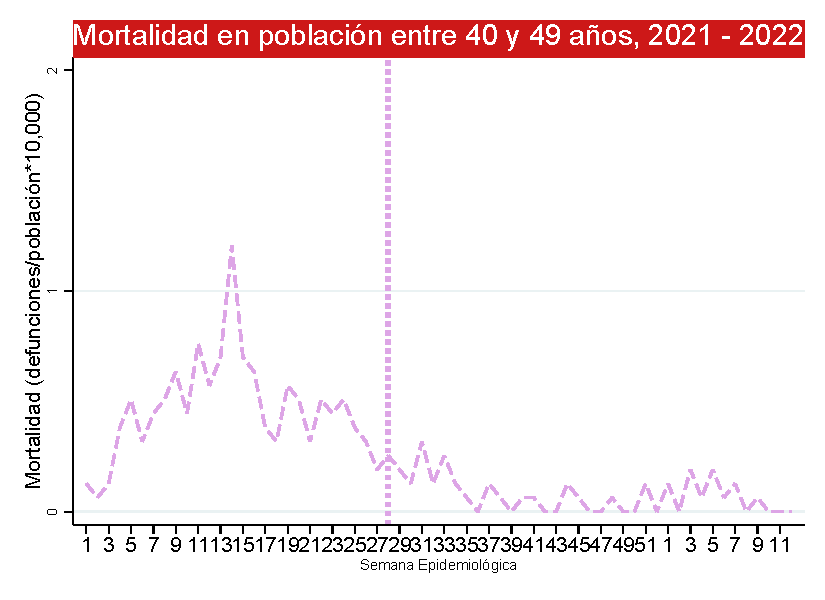
\includegraphics[width=\textwidth]{../figuras/mortalidad_edad_40.pdf}
		\caption{40 a 49 años}
		%\label{fig:40 a 49 años}
	\end{subfigure}
	\hfill
	\begin{subfigure}[b]{0.45\textwidth}
		\centering
		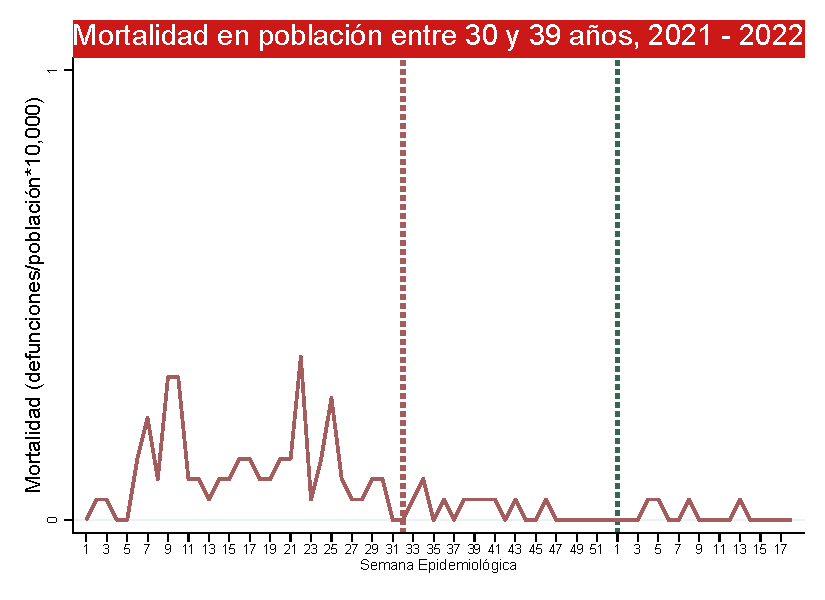
\includegraphics[width=\textwidth]{../figuras/mortalidad_edad_30.pdf}
		\caption{30 a 39 años}
		%\label{fig:40 a 49 años}
	\end{subfigure}
	\end{figure}

\clearpage
	
	\subsection*{Exceso de Muertes por Todas las Causas}
	\noindent  La Figura \ref{fig:exceso_regional} muestra la tendencia del exceso de muertes con respecto al año 2019. Para la SE 47, el exceso de muertes en el año 2021 presentó una pendiente en descenso comparada con respecto al año 2019, lo que se traduce en un Exceso de muerte negativo (menos 10). Es decir, para esta semana hubieron menos muertes a comparación del año 2019.   

	\begin{figure}[h]
	\caption{Exceso de Fallecidos por  Todas las Causa en la Región Cusco,  hasta la SE 47 - 2021.}\label{fig:exceso_regional}
	\begin{center}
		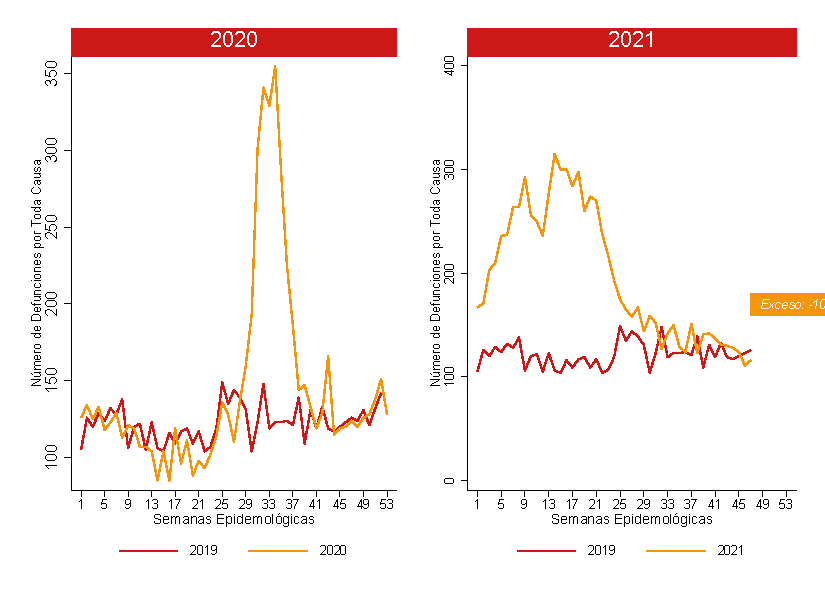
\includegraphics[width=0.85\linewidth]{../figuras/exceso_region.pdf}
	\end{center}
	{\footnotesize {Fuente de datos: SISCOVID, NOTICOVID.}}
	\end{figure}
\clearpage

	\subsection*{Cobertura de Vacunación por COVID-19 en la Región Cusco, hasta la SE 47.}
\noindent La Figura \ref{fig:vacuna_edad} muestra la cobertura de vacunación por grupo etario en la Región Cusco. El mayor porcentaje de cobertura se encuentra en el grupo etario de 50 a 59 años (con 77$\%$ de personas con dos dosis de vacuna), seguido del grupo etario de 60 a 69 años  (con 75,9$\%$ de personas con dos dosis de vacuna). El menor cobertura de vacunación se encuentra en el grupo etario de 12 a 19 años, con 38,9$\%$ de personas vacunadas con las dos dosis. 

\begin{figure}[h]
	\caption{Cobertura de Vacunación por Grupo Etario en la Región Cusco, hasta la SE 47. }\label{fig:vacuna_edad}
	\begin{center}
		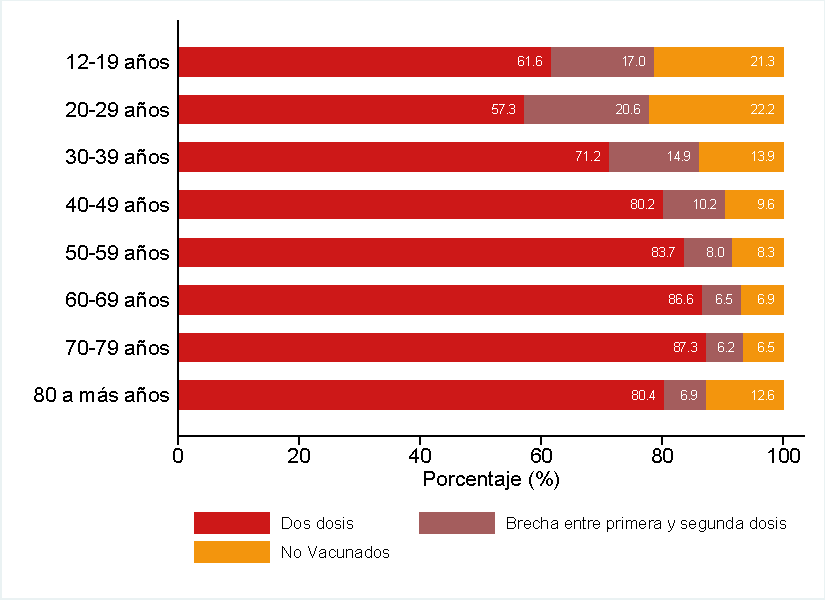
\includegraphics[width=0.65\linewidth]{../figuras/vacunacion_grupo_edad.pdf}
	\end{center}
	{\footnotesize {Fuente de datos: SICOVAC, HIS-MINSA.}}
\end{figure}

La Figura \ref{fig:cobertura_vacunaci_provincia}  muestra la cobertura de vacunación en cada una de las provincias de Cusco por grupo etario. Es preciso señalar que la provincia de Espinar tiene la cobertura más baja de la región, en los grupos etarios desde los 50 años en adelante.

\begin{figure}[h]
	\caption{Cobertura de Vacunación por Provincia y por Grupo Etario en la Región Cusco, hasta la SE 47.}
	\label{fig:cobertura_vacunaci_provincia}
	\centering
	\begin{subfigure}[b]{0.45\textwidth}
		\centering
		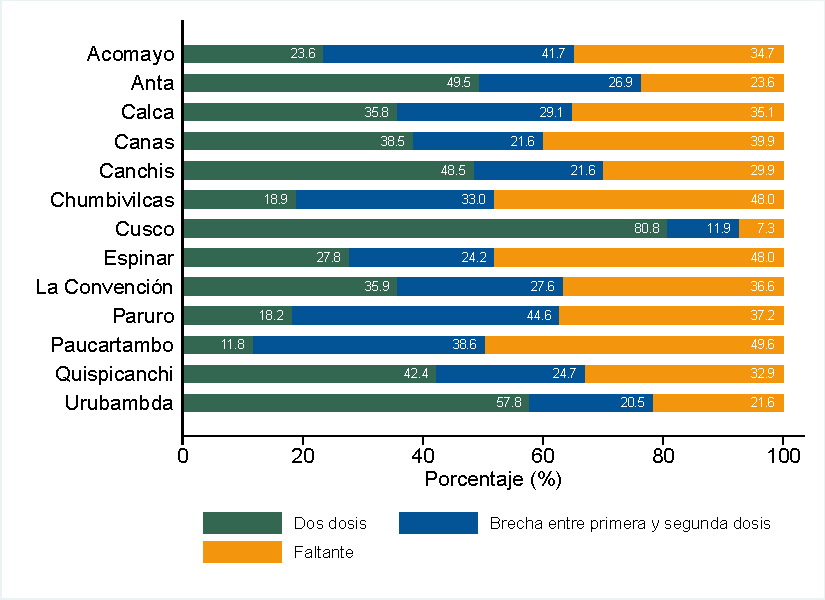
\includegraphics[width=\textwidth]{../figuras/vacunacion_provincial_edad_1}
		\caption{ De 12 a 19 años}
		%\label{fig:}
	\end{subfigure}
	\hfill
	\begin{subfigure}[b]{0.45\textwidth}
		\centering
		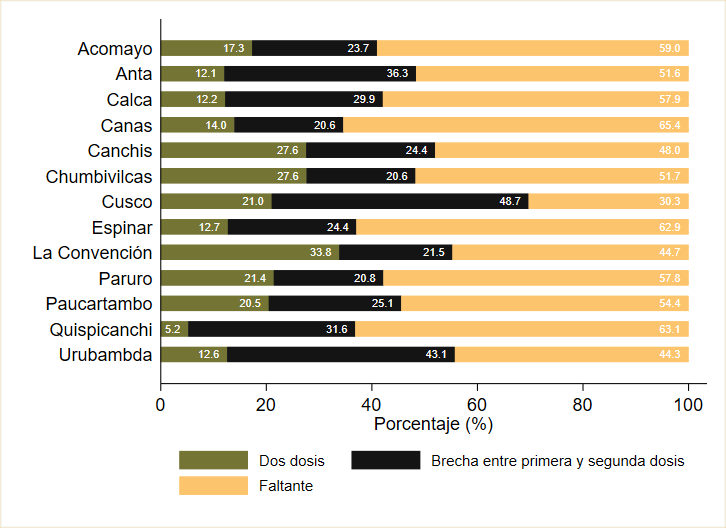
\includegraphics[width=\textwidth]{../figuras/vacunacion_provincial_edad_2}
		\caption{De 20 a 29 años}
		%\label{fig:70 a 79 años}
	\end{subfigure}
	\begin{subfigure}[b]{0.45\textwidth}
		\centering
		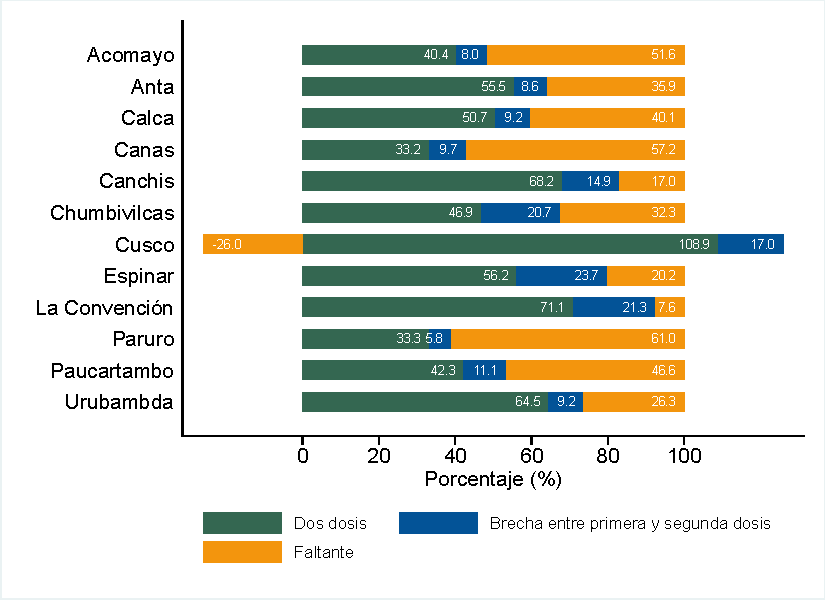
\includegraphics[width=\textwidth]{../figuras/vacunacion_provincial_edad_3}
		\caption{De 30 a 39 años}
		%\label{fig:60 a 69 años}
	\end{subfigure}
	\hfill
	\begin{subfigure}[b]{0.45\textwidth}
		\centering
		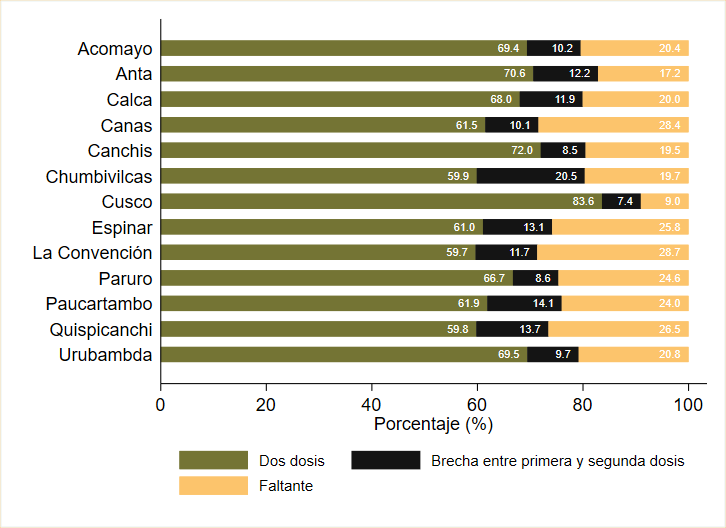
\includegraphics[width=\textwidth]{../figuras/vacunacion_provincial_edad_4}
		\caption{De 40 a 49 años}
		%\label{fig:50 a 59 años}
	\end{subfigure}
	\begin{subfigure}[b]{0.45\textwidth}
		\centering
		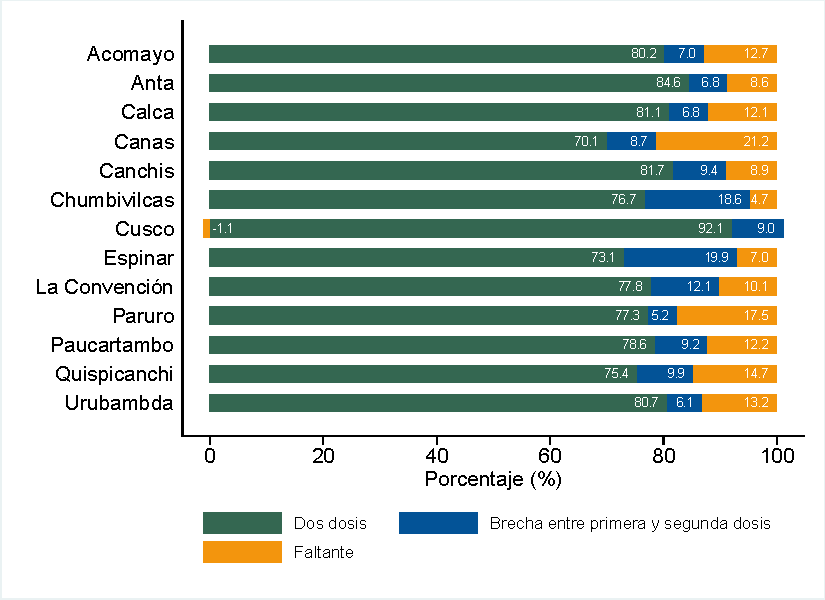
\includegraphics[width=\textwidth]{../figuras/vacunacion_provincial_edad_5}
		\caption{De 50 a 59 años}
		%\label{fig:40 a 49 años}
	\end{subfigure}
	\hfill
	\begin{subfigure}[b]{0.45\textwidth}
		\centering
		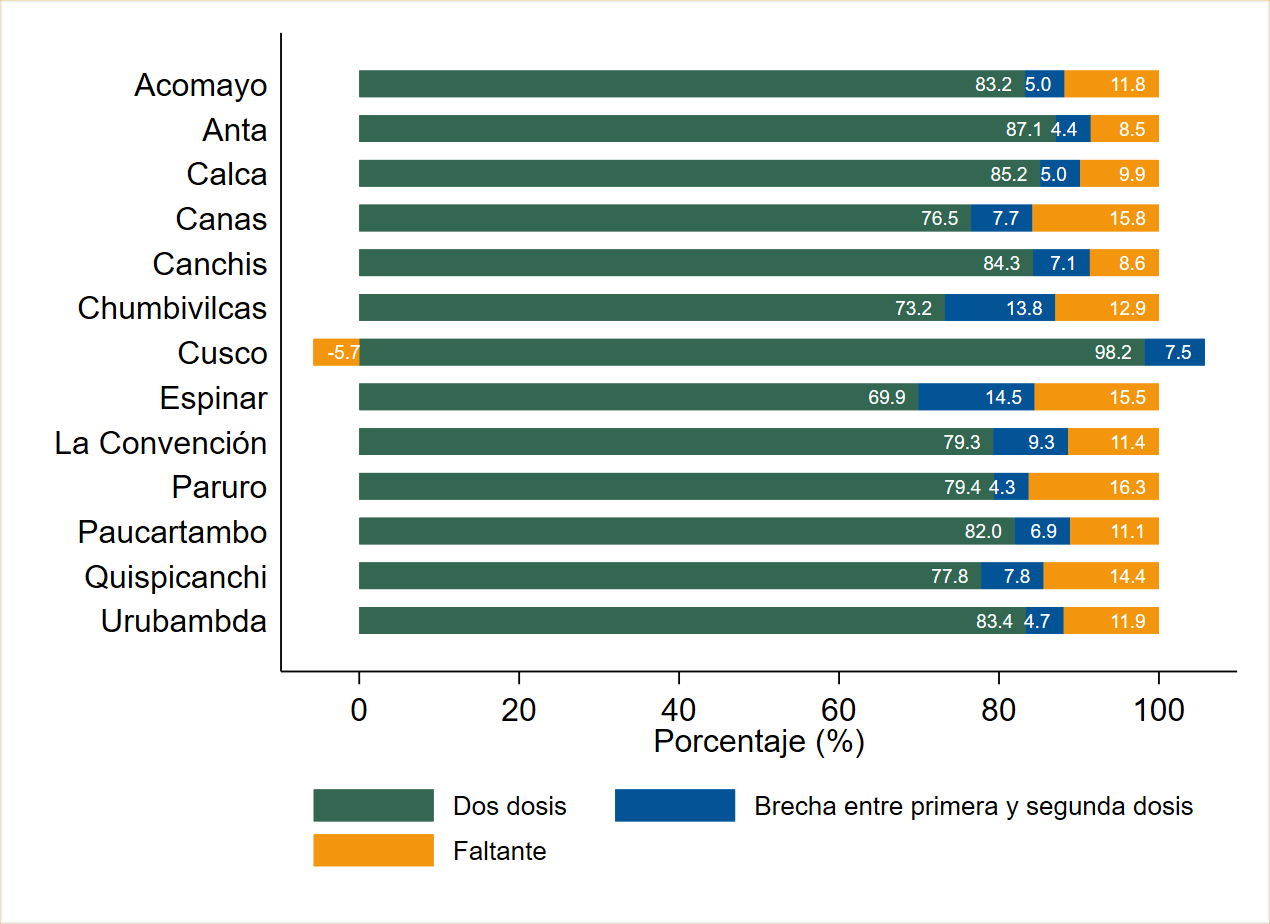
\includegraphics[width=\textwidth]{../figuras/vacunacion_provincial_edad_6}
		\caption{De 60 a 69 años}
		%\label{fig:40 a 49 años}
	\end{subfigure}
\begin{subfigure}[b]{0.45\textwidth}
	\centering
	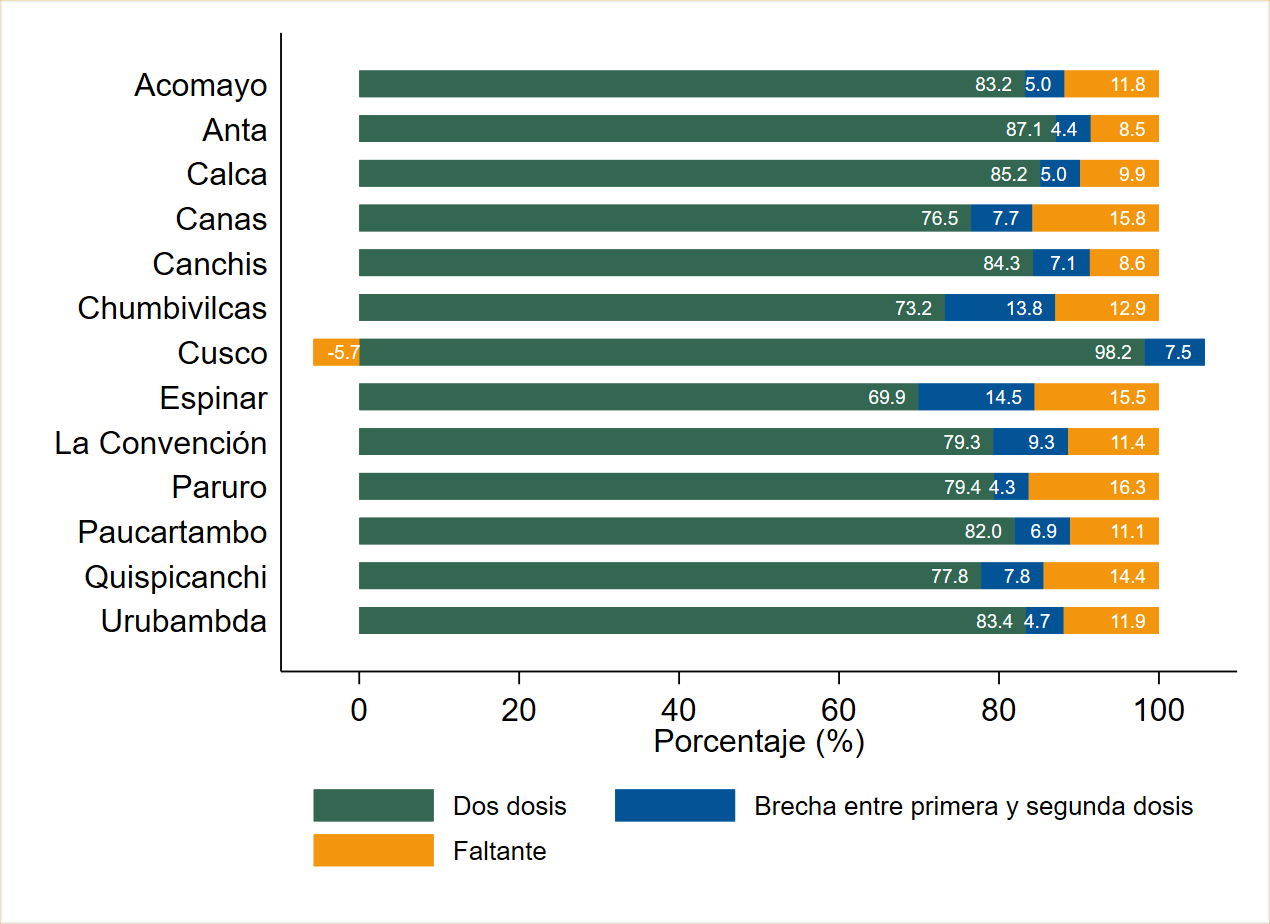
\includegraphics[width=\textwidth]{../figuras/vacunacion_provincial_edad_6}
	\caption{De 70 a 79 años}
	%\label{fig:40 a 49 años}
\end{subfigure}
\hfill
\begin{subfigure}[b]{0.45\textwidth}
	\centering
	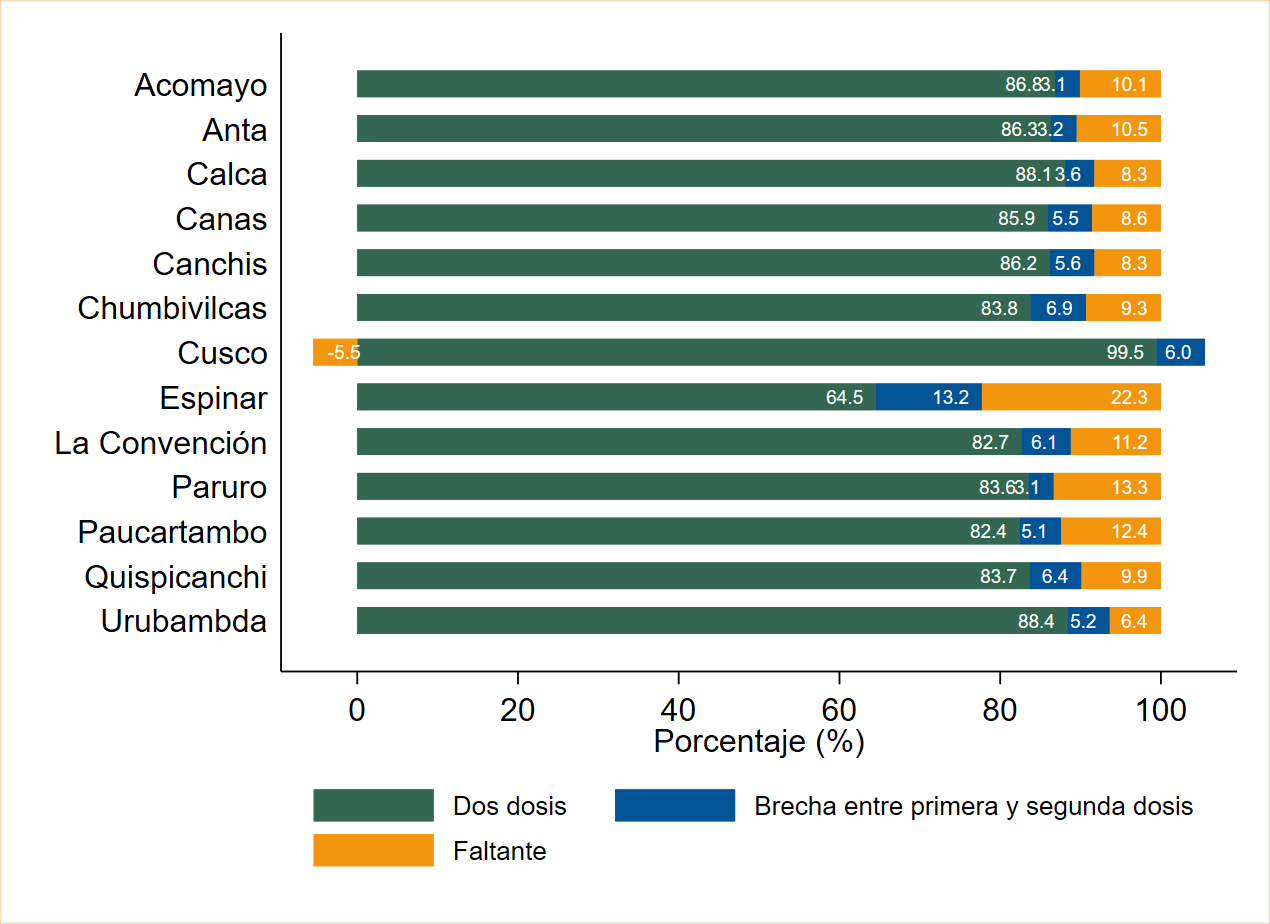
\includegraphics[width=\textwidth]{../figuras/vacunacion_provincial_edad_7}
	\caption{Más de 80 años}
	%\label{fig:40 a 49 años}
\end{subfigure}
\end{figure}

\clearpage
\subsection*{Ocupación de Camas}
\noindent La disponibilidad y ocupación de camas UCI se ve resumida en la Figura \ref{fig:ocupacion_uci}, se evidencia que para la SE 46, el número de camas UCI decreció a 32 (siete camas menos respecto a las semanas anteriores), sin embargo el porcentaje de ocupación no sufrió variaciones considerables, para la SE el porcentaje de ocupación es del 75$\%$. 

\begin{figure}[h]
	\caption{Ocupación de Camas UCI COVID-19 en la Región Cusco, hasta la SE 47, 2021.}\label{fig:ocupacion_uci}
	\begin{center}
		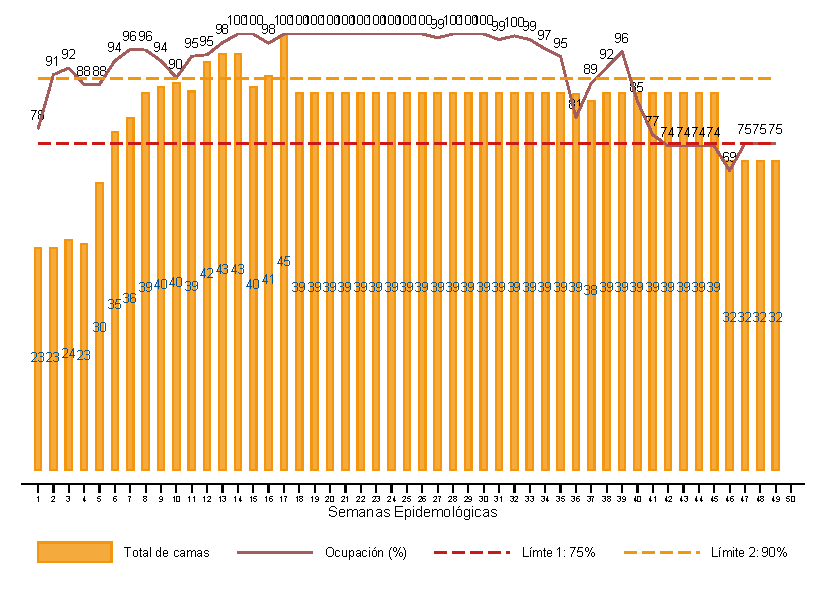
\includegraphics[width=0.95\linewidth]{../figuras/uci.pdf}
	\end{center}
	{\footnotesize {Fuente de datos: REFERENCIAS Y CONTRAREFERENCIAS.}}
\end{figure}
\cleardoublepage

En la Figura \ref{fig:ocupacion_3_nivel}, se plasma el porcentaje de ocupación y número de camas no-UCI COVID en el nivel Hospitalario III. Para la SE 46, el número de camas descendió a 267, sin embargo el porcentaje de ocupación se mantiene bajo, quedando alrededor de 87$\%$ de camas disponibles para hospitalización. 
  
\begin{figure}[htpb]
	\caption{Ocupación de Camas no UCI COVID-19 en el nivel III en la Región Cusco, hasta la SE 47, 2021.}\label{fig:ocupacion_3_nivel}
	\begin{center}
		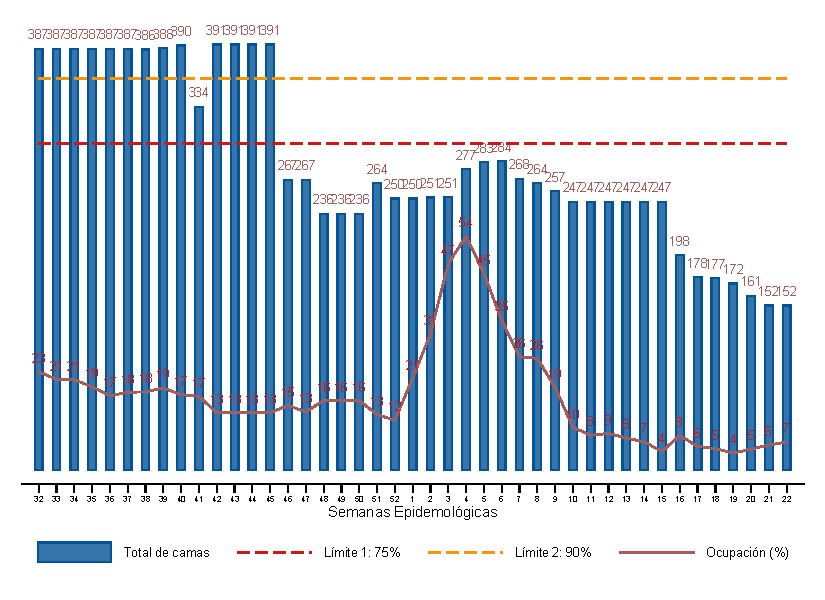
\includegraphics[width=0.95\linewidth]{../figuras/nivel_3.pdf}
	\end{center}
	{\footnotesize {Fuente de datos: REFERENCIAS Y CONTRAREFERENCIAS.}}
\end{figure}

\clearpage

En la Figura \ref{fig:ocupacion_2nivel}, se observa el número de camas disponibles y su porcentaje de ocupación en el Nivel II. Se evidencia que el porcentaje de ocupación de camas tiene una tendencia al descenso, siendo sólo del 6$\%$ para la SE 47. 

\begin{figure}[h]
	\caption{Disponibilidad y Ocupación de Camas-COVID a Nivel de Hospitales del Nivel II en la Región Cusco, hasta la SE 47, 2021}\label{fig:ocupacion_2nivel}
	\begin{center}
		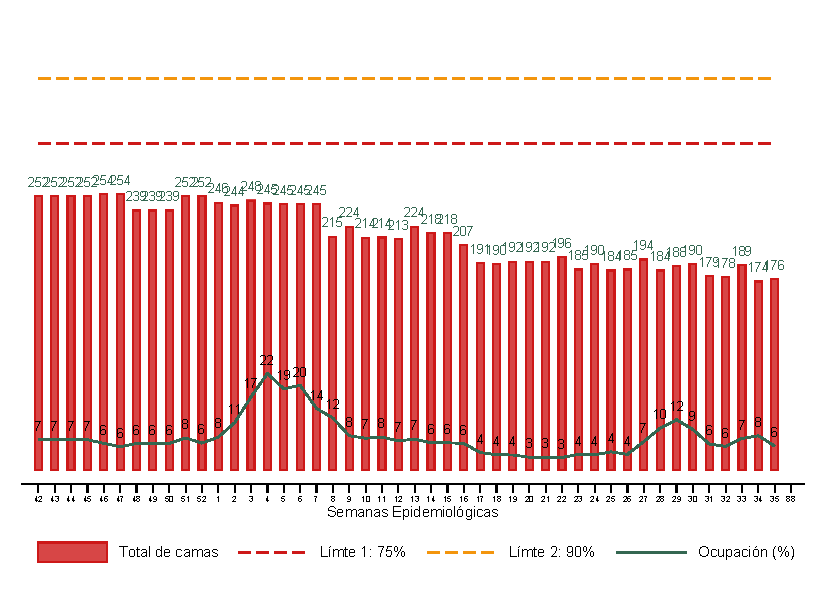
\includegraphics[width=0.95\linewidth]{../figuras/nivel_2.pdf}
	\end{center}
	{\footnotesize {Fuente de datos: REFERENCIAS Y CONTRAREFERENCIAS.}}
\end{figure}
\clearpage
\begin{landscape}
	
	\subsection*{Evaluación Provincial de la Infección por COVID-19} 
	
	\begin{tabular}{@{}lrrrrr@{}}
	\rowcolor[HTML]{ECF4FF} 
	\textbf{Provincias}                   & \multicolumn{1}{l}{\cellcolor[HTML]{ECF4FF}\textbf{población}} & \multicolumn{1}{l}{\cellcolor[HTML]{ECF4FF}\textbf{Pruebas Totales}} & \multicolumn{1}{l}{\cellcolor[HTML]{ECF4FF}\textbf{Funciones}} & \multicolumn{1}{l}{\cellcolor[HTML]{ECF4FF}\textbf{Tasa de letalidad}} & \multicolumn{1}{l}{\cellcolor[HTML]{ECF4FF}\textbf{\begin{tabular}[c]{@{}l@{}}tasa de mortalidad x \\   100.000 hab\end{tabular}}} \\
	\cellcolor[HTML]{FD6864}CANCHIS       & 105,049                                                        & 1,545                                                                & 5                                                              & 0.3\%                                                                  & 4.8                                                                                                                                \\
	\cellcolor[HTML]{FD6864}PAUCARTAMBO   & 52,989                                                         & 301                                                                  & 2                                                              & 0.7\%                                                                  & 3.8                                                                                                                                \\
	\cellcolor[HTML]{FD6864}LA CONVENCION & 185,793                                                        & 2,623                                                                & 7                                                              & 0.3\%                                                                  & 3.8                                                                                                                                \\
	\cellcolor[HTML]{FFFC9E}CUSCO         & 463,656                                                        & 16,911                                                               & 9                                                              & 0.1\%                                                                  & 1.9                                                                                                                                \\
	\cellcolor[HTML]{FFFC9E}ESPINAR       & 71,304                                                         & 479                                                                  & 1                                                              & 0.2\%                                                                  & 1.4                                                                                                                                \\
	\cellcolor[HTML]{FFFC9E}CALCA         & 76,462                                                         & 462                                                                  & 1                                                              & 0.2\%                                                                  & 1.3                                                                                                                                \\
	\cellcolor[HTML]{9AFF99}CHUMBIVILCAS  & 84,925                                                         & 448                                                                  & 1                                                              & 0.2\%                                                                  & 1.2                                                                                                                                \\
	\cellcolor[HTML]{9AFF99}QUISPICANCHI  & 92,566                                                         & 735                                                                  & 1                                                              & 0.1\%                                                                  & 1.1                                                                                                                                \\
	\cellcolor[HTML]{9AFF99}ACOMAYO       & 28,477                                                         & 149                                                                  & 0                                                              & 0.0\%                                                                  & 0.0                                                                                                                                \\
	\cellcolor[HTML]{9AFF99}ANTA          & 57,731                                                         & 480                                                                  & 0                                                              & 0.0\%                                                                  & 0.0                                                                                                                                \\
	\cellcolor[HTML]{9AFF99}CANÁS         & 40,420                                                         & 206                                                                  & 0                                                              & 0.0\%                                                                  & 0.0                                                                                                                                \\
	\cellcolor[HTML]{9AFF99}PARURO        & 31,264                                                         & 132                                                                  & 0                                                              & 0.0\%                                                                  & 0.0                                                                                                                                \\
	\cellcolor[HTML]{9AFF99}URUBAMBÁ      & 66,439                                                         & 900                                                                  & 0                                                              & 0.0\%                                                                  & 0.0                                                                                                                                \\
	& \multicolumn{1}{l}{}                                           & \multicolumn{1}{l}{}                                                 & \multicolumn{1}{l}{}                                           & \multicolumn{1}{l}{}                                                   & \multicolumn{1}{l}{}                                                                                                               \\
	\rowcolor[HTML]{ECF4FF} 
	\textbf{Totales generales}            & \textbf{1,357,075}                                             & \textbf{25,371}                                                      & \textbf{27}                                                    & \textbf{0.11\%}                                                        & \textbf{2.0}                                                                                                                      
\end{tabular}
	{\footnotesize Fuente de datos: NOTICOVID, SISCOVID, SINADEF.}
	
	\noindent El Cuadro muestra la tasa de letalidad y mortalidad de todas las provincias de la Región Cusco. Se presentan las provincias ordenadas de mayor a menor tasa de mortalidad, encontrándose la mayor tasa (278.9 defunciones/ 100 000 habitantes) en Canchis. 
	
\end{landscape}
%---------------------------------------------------------------------------
% CAPÍTULO: EVALUACIÓN DE PROVINCIAS
%---------------------------------------------------------------------------

%insertar el cover del capitulo
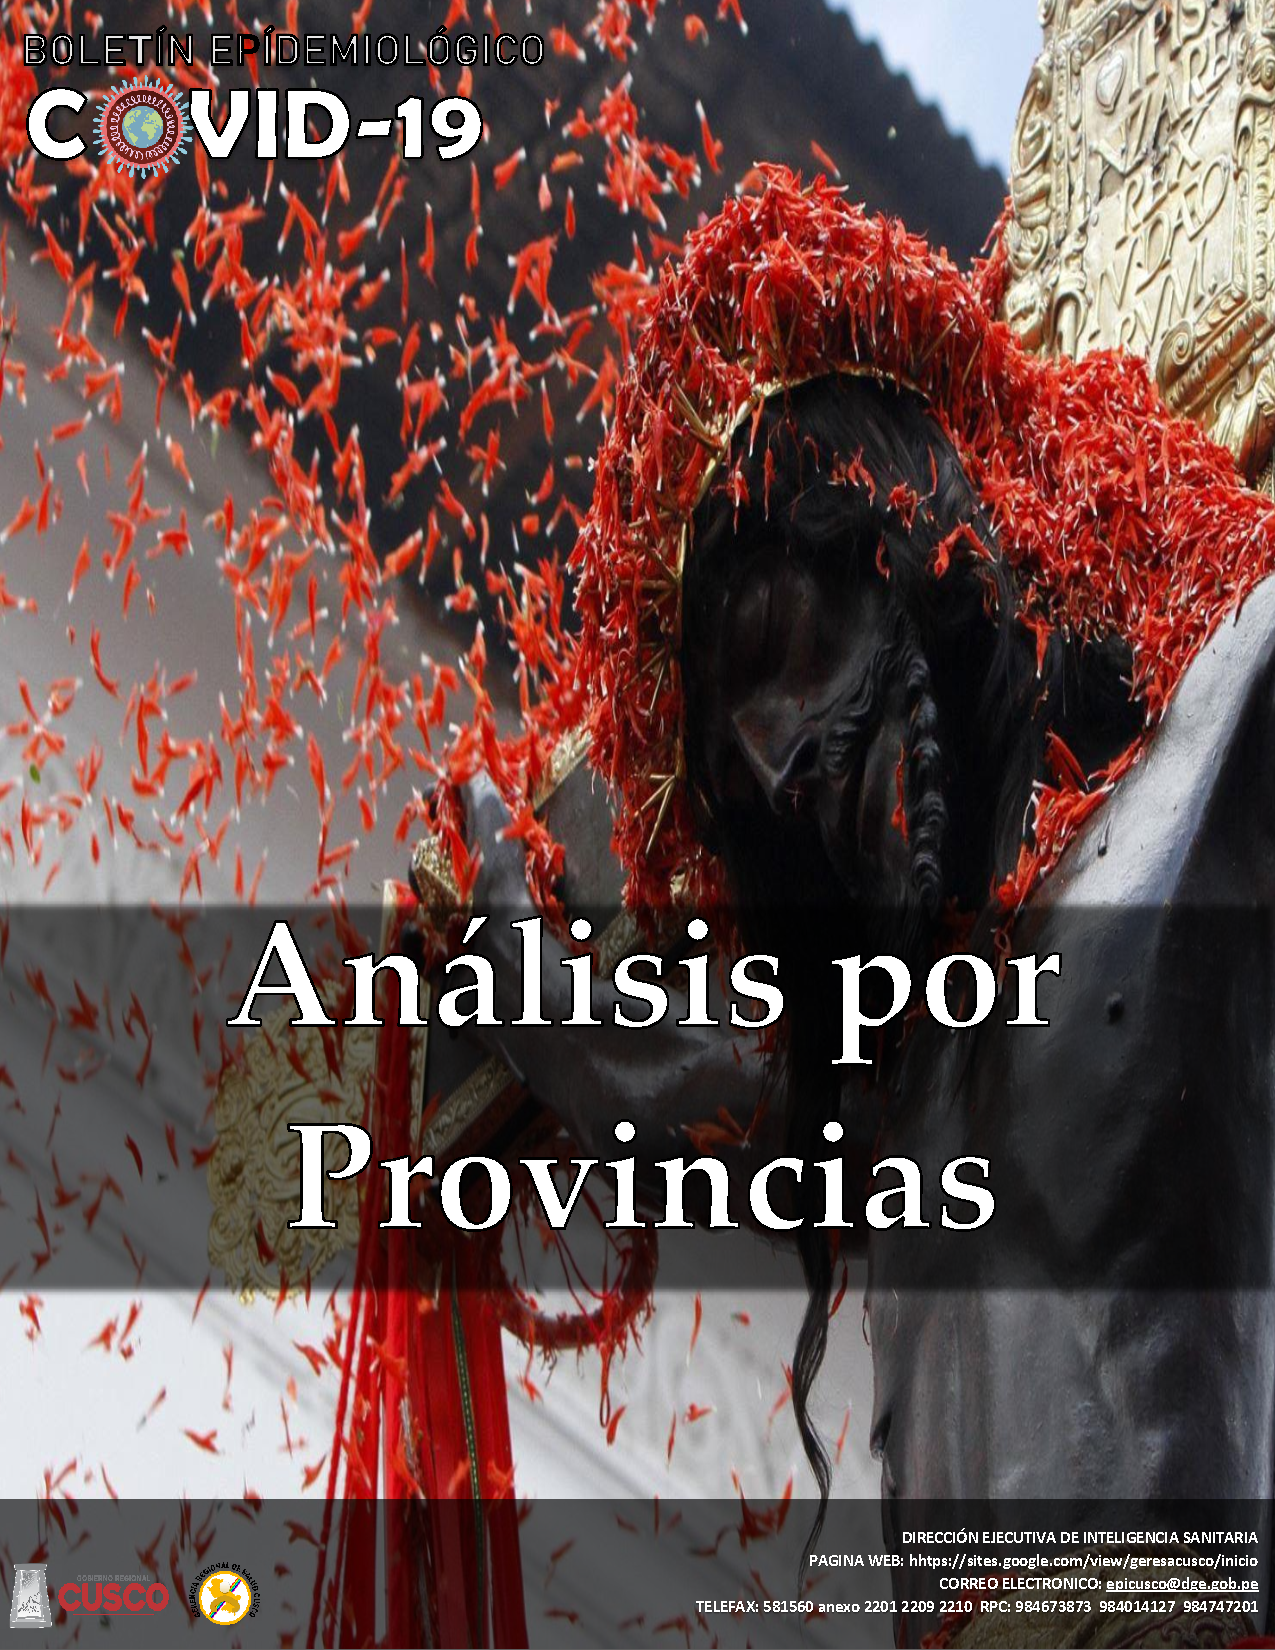
\includepdf[pages={1}]{../editorial/5.pdf}
\clearpage

	\section*{Evaluación para Provincias Priorizadas}
\addcontentsline{toc}{chapter}{Evaluación para Provincias Priorizadas}
\noindent La Figura \ref{fig:incidencia_provincias} muestra las tasas de incidencia acumulada por provincia de Cusco ordenadas de mayor a menor incidencia acumulada. Se observa que la provincia de Cusco tiene la tasa de incidencia acumulada más alta (944.4 casos /10 000* personas), seguida de la provincia de La Convención (584,7 casos/10 000*personas).

\begin{figure}[!htpb]
	\caption{Tasa de Incidencia Acumulada por Provincia en la Región Cusco, hasta el 27 de noviembre del 2021. }\label{fig:incidencia_provincias}
	\begin{center}
		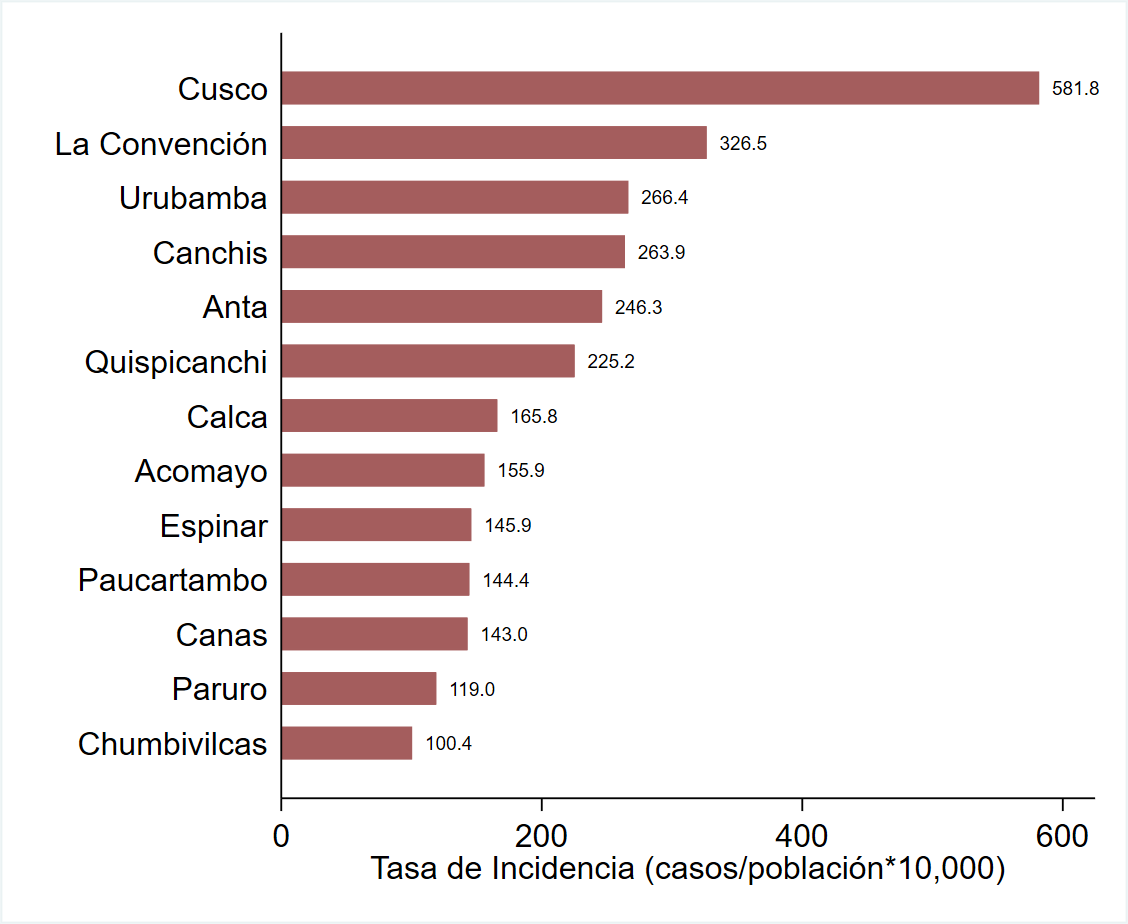
\includegraphics[width=0.75\linewidth]{../figuras/incidencia_provincial}
	\end{center}
	{\footnotesize {Fuente de datos: SISCOVID, NOTICOVID.}}
\end{figure}


La Figura \ref{fig:mortalidad_ordenada} muestra a las provincias de la Región ordenadas de mayor a menor Tasa de Mortalidad Acumulada. Se evidencia que la provincia de Canchis continúa como provincia con mayor Tasa de Mortalidad Acumulada con 28 defunciones / 10 000* personas.  

\begin{figure}[h]
	\caption{Tasa de Mortalidad Acumulada por Provincia en la Región Cusco, hasta el 27 de noviembre del 2021. }\label{fig:mortalidad_ordenada}
	\begin{center}
		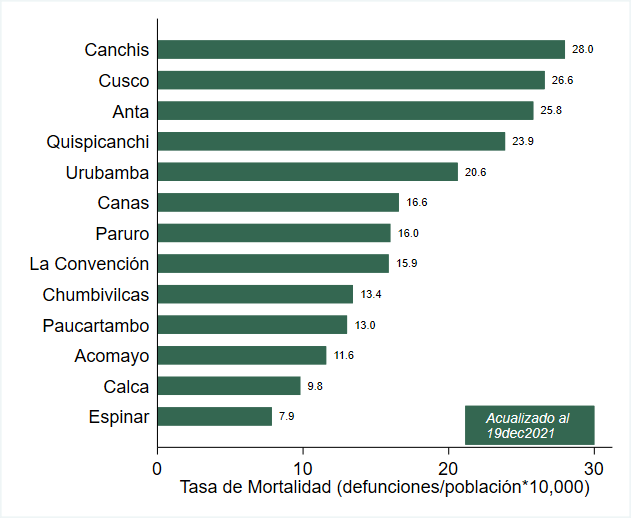
\includegraphics[width=0.65\linewidth]{../figuras/mortalidad_provincial}
	\end{center}
	{\footnotesize {Fuente de datos: SISCOVID, NOTICOVID.}}
\end{figure}

La Figura \ref{fig:incidencia_provincial} muestra la tendencia de la Incidencia acumulada a través del año. En las últimas dos semanas, la pendiente se crecimiento se ha mantenido en meceta. 
%
\begin{figure}[h]
	\caption{Tendencia Provincial de Incidencia acumulada de COVID-19, hasta la SE 47, 2021. }\label{fig:incidencia_provincial}
	\begin{center}
		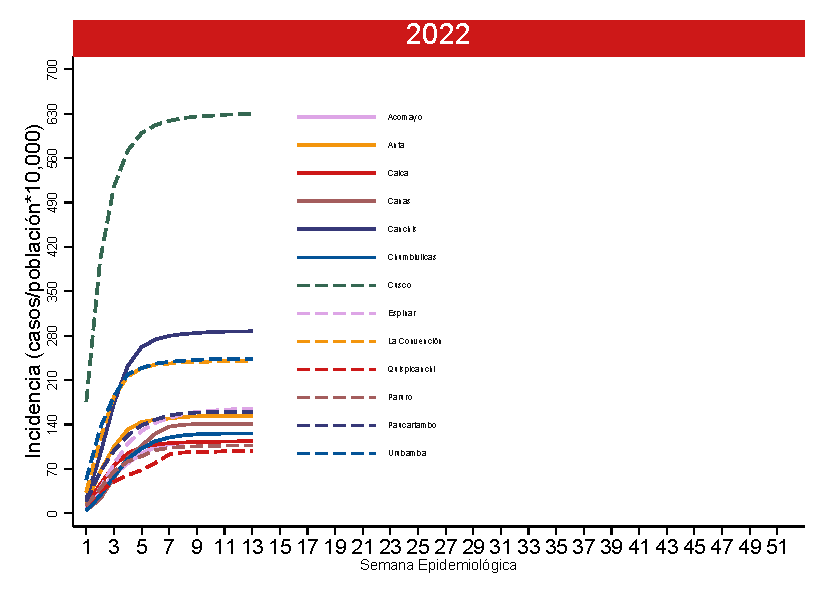
\includegraphics[width=0.65\linewidth]{../figuras/incidencia_provincial_2021.pdf}
	\end{center}
	{\footnotesize {Fuente de datos: SINADEF.}}
\end{figure}

\clearpage
	
\section*{Evaluación Provincial de 5 Indicadores}
		\noindent El objetivo de estas figuras es comparar a cada provincia consigo misma de acuerdo a su historia  en la primera ola (en el año 2020). Se evaluaron los siguientes indicadores: incidencia, tasa de mortalidad, tasa de positividad por prueba molecular, tasa de positividad por prueba antigénica, y exceso de defunciones para cada provincia.
		
		\subsection*{Provincia de Acomayo}
		\noindent Las figuras inferiores (Figura \ref{fig:inc_mort_acomayo}, \ref{fig:positividad_acomayo}) muestra un comportamiento variable de la mortalidad a lo largo del años, presentando una disminución marcada desde la SE 37. En la Figura \ref{fig:exceso_acomayo} se muestra que hay un exceso de menos 3 defunciones respecto al año 2020.
		
		\begin{figure}[h]
			\caption{Tasa de Incidencia y Mortalidad Comparativa en la Provincia de Acomayo 2020 y 2021, hasta la SE 43. }\label{fig:inc_mort_acomayo}
			\begin{center}
				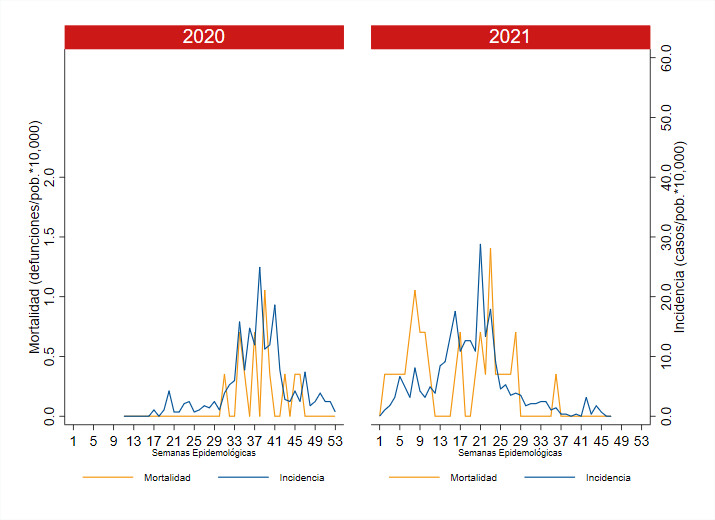
\includegraphics[width=0.7\linewidth]{../figuras/incidencia_mortalidad_20_21_1}
			\end{center}
			{\footnotesize {Fuente de datos: NOTICOVID, SISCOVID, SINADEF.}}
		\end{figure}
		
		\begin{figure}[h]
			\caption{Tasa de Positividad de Prueba Molecular y Antigénica Comparativa en la Provincia de Acomayo 2020 y 2021, hasta la SE 43. }\label{fig:positividad_acomayo}
			\begin{center}
				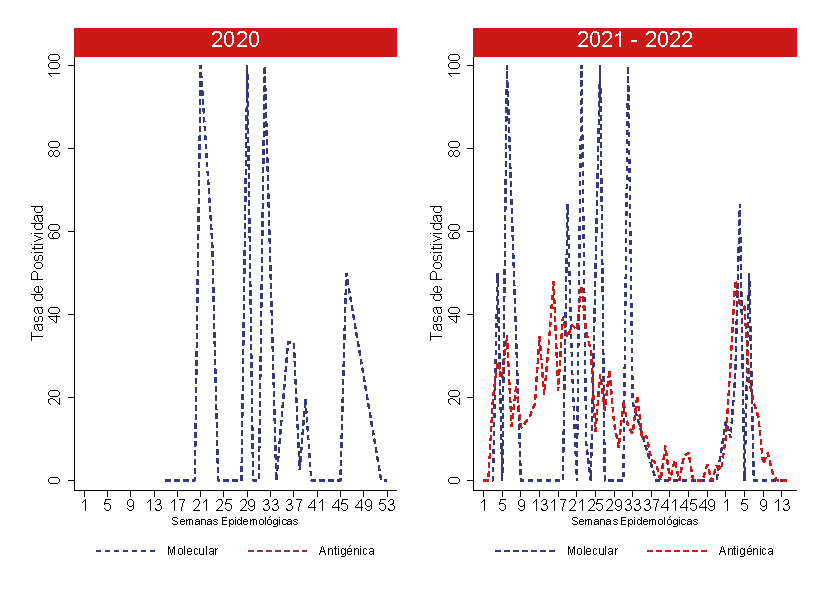
\includegraphics[width=0.7\linewidth]{../figuras/positividad_20_21_1}
			\end{center}
			{\footnotesize {Fuente de datos: NOTICOVID, SISCOVID.}}
		\end{figure}
		
		\begin{figure}[h]
			\caption{Exceso de Defunciones Comparativo en la Provincia de Acomayo 2020 y 2021, hasta la SE 43.}\label{fig:exceso_acomayo}
			\begin{center}
				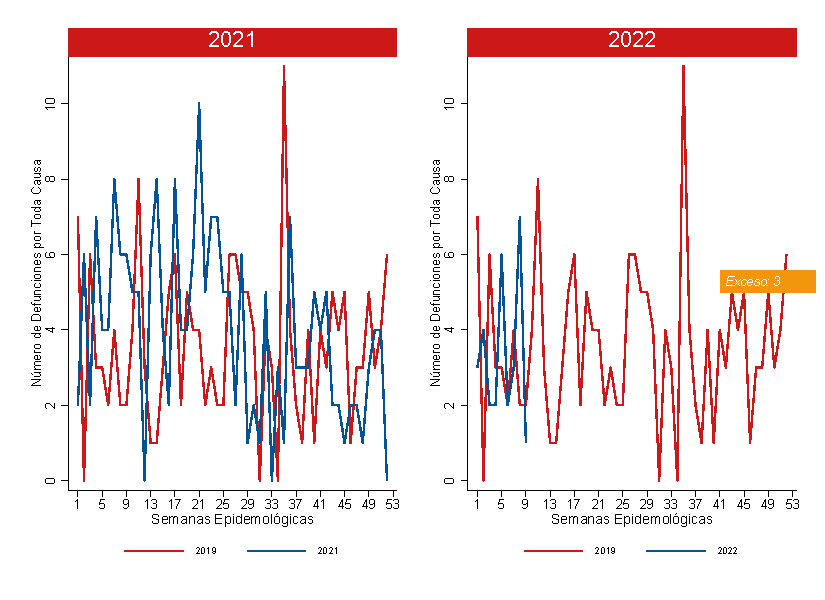
\includegraphics[width=0.7\linewidth]{../figuras/exceso_1}
			\end{center}
			{\footnotesize {Fuente de datos: SINADEF.}}
		\end{figure}
		
		% Anta
		\clearpage
		
		\subsection*{Provincia de Anta}
		\noindent Las figuras de abajo (Figura \ref{fig:inc_mort_anta}, \ref{fig:positividad_anta})  muestra una discreto aumento en la incidencia de casos de COVID-19, con respecto a la mortalidad, ésta se  ha mantenido variable el tiempo. En la Figura \ref{fig:exceso_anta} se muestra que no hay exceso de defunciones respecto al año 2020.
		
		\begin{figure}[h]
			\caption{Tasa de Incidencia y Mortalidad Comparativa en la Provincia de Anta 2020 y 2021, hasta la SE 43.}\label{fig:inc_mort_anta}
			\begin{center}
				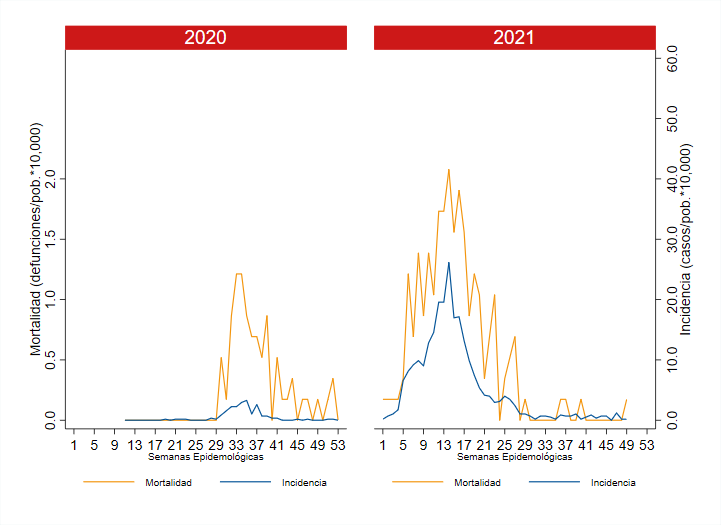
\includegraphics[width=0.7\linewidth]{../figuras/incidencia_mortalidad_20_21_2}
			\end{center}
			{\footnotesize {Fuente de datos: NOTICOVID, SISCOVID, SINADEF.}}
		\end{figure}
		
		\begin{figure}[h]
			\caption{Tasa de Positividad de Prueba Molecular y Antigénica Comparativa en la Provincia de Anta 2020 y 2021, hasta la SE 43.}\label{fig:positividad_anta}
			\begin{center}
				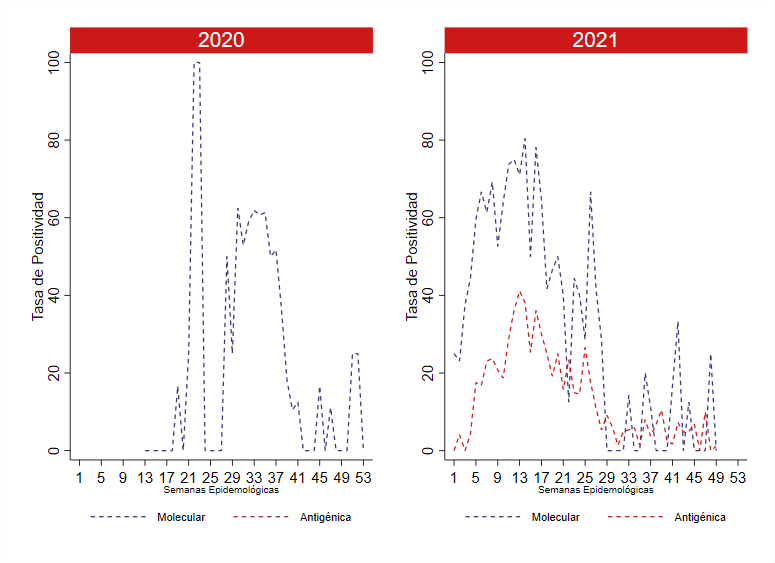
\includegraphics[width=0.7\linewidth]{../figuras/positividad_20_21_2}
			\end{center}
			{\footnotesize {Fuente de datos: NOTICOVID, SISCOVID.}}
		\end{figure}
		
		\begin{figure}[h]
			\caption{Exceso de Defunciones Comparativo en la Provincia de Anta  2020 y 2021, hasta la SE 43.}\label{fig:exceso_anta}
			\begin{center}
				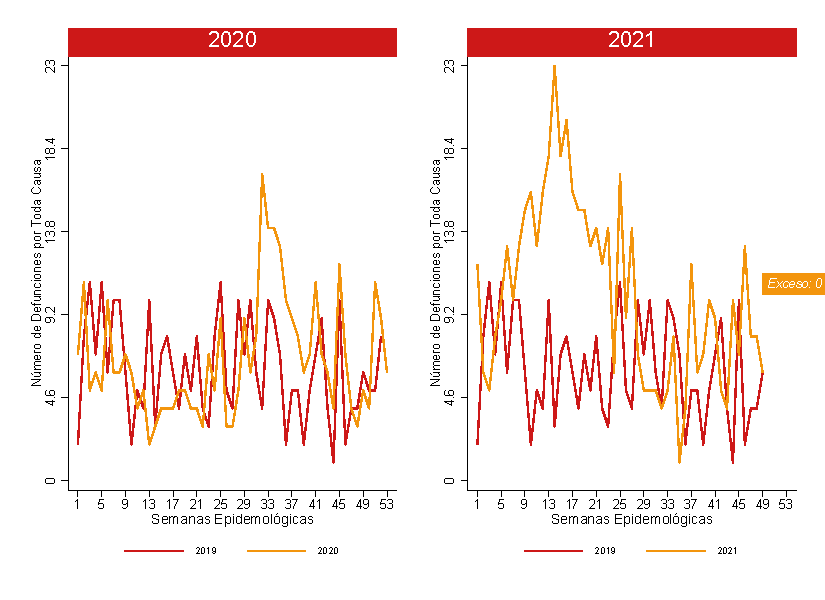
\includegraphics[width=0.7\linewidth]{../figuras/exceso_2}
			\end{center}
			{\footnotesize {Fuente de datos: SINADEF.}}
		\end{figure}
		
		% Canas
		\clearpage
		
		\subsection*{Provincia de Canas}
		\noindent Las figuras de abajo (Figura \ref{fig:inc_mort_canas}, \ref{fig:positividad_canas}) se muestra un incremento discreto pero sostenido de la tasa de Incidencia de COVID-19 en la provincia de Canas, con respecto a la mortalidad no se registraron muertes desde la SE 38. En la Figura \ref{fig:exceso_canas} se muestra que hay un exceso de menos 5 defunciones respecto al año 2020.
		
		\begin{figure}[h]
			\caption{Tasa de Incidencia y Mortalidad Comparativa en la Provincia de Canas 2020 y 2021, hasta la SE 43.}\label{fig:inc_mort_canas}
			\begin{center}
				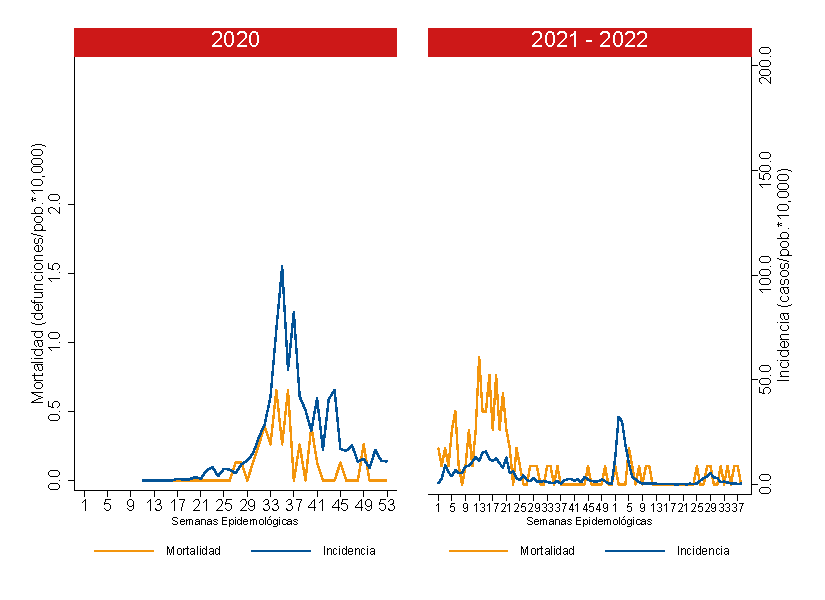
\includegraphics[width=0.7\linewidth]{../figuras/incidencia_mortalidad_20_21_3}
			\end{center}
			{\footnotesize {Fuente de datos: NOTICOVID, SISCOVID, SINADEF.}}
		\end{figure}
		
		\begin{figure}[h]
			\caption{Tasa de Positividad de Prueba Molecular y Antigénica Comparativa en la Provincia de Canas 2020 y 2021, hasta la SE 43.}\label{fig:positividad_canas}
			\begin{center}
				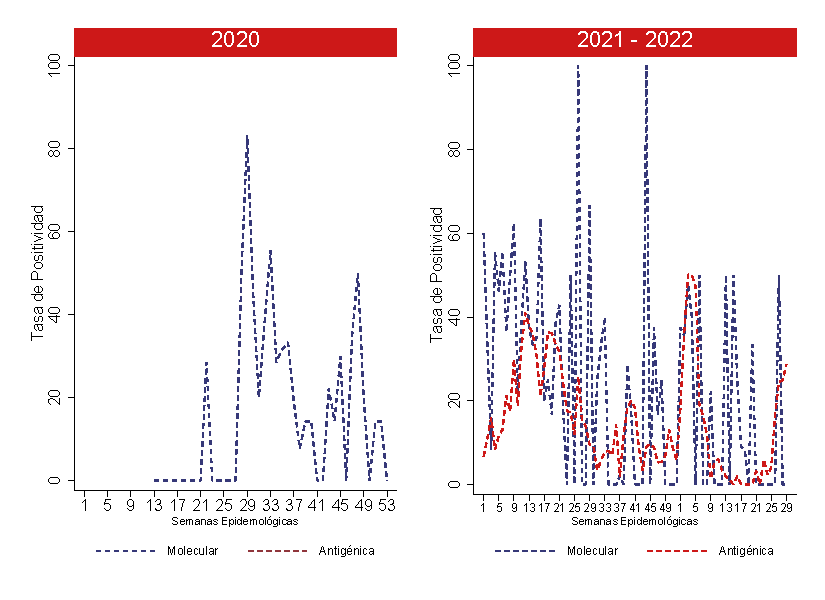
\includegraphics[width=0.7\linewidth]{../figuras/positividad_20_21_3}
			\end{center}
			{\footnotesize {Fuente de datos: NOTICOVID, SISCOVID.}}
		\end{figure}
		
		\begin{figure}[h]
			\caption{Exceso de Defunciones Comparativo en la Provincia de Canas 2020 y 2021, hasta la SE 43.}\label{fig:exceso_canas}
			\begin{center}
				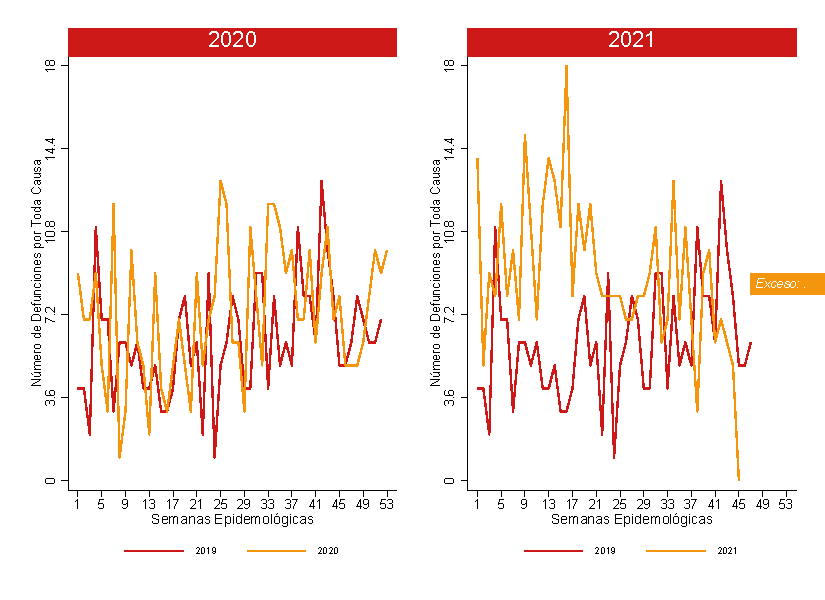
\includegraphics[width=0.7\linewidth]{../figuras/exceso_3}
			\end{center}
			{\footnotesize {Fuente de datos: SINADEF.}}
		\end{figure}
		
		% Calca
		\clearpage
		
		\subsection*{Provincia de Calca}
		\noindent Las figuras de abajo (Figura \ref{fig:inc_mort_calca}, \ref{fig:positividad_calca}) muestra que tantao la tasa de mortalidad como la de la incidencia se ha mantenido variable desde la SE 41, con picos entre semanas. En la Figura \ref{fig:exceso_calca} se muestra que hay un exceso de menos 2 defunciones respecto al año 2020.
		
		\begin{figure}[h]
			\caption{Tasa de Incidencia y Mortalidad Comparativa en la Provincia de Canas 2020 y 2021, hasta la SE 43.}\label{fig:inc_mort_calca}
			\begin{center}
				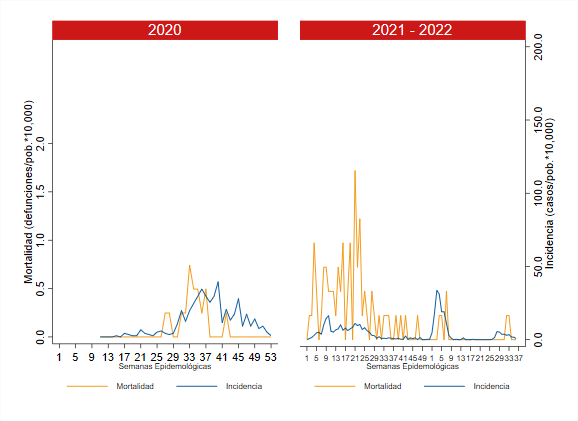
\includegraphics[width=0.7\linewidth]{../figuras/incidencia_mortalidad_20_21_4}
			\end{center}
			{\footnotesize {Fuente de datos: NOTICOVID, SISCOVID, SINADEF.}}
		\end{figure}
		
		\begin{figure}[h]
			\caption{Tasa de Positividad de Prueba Molecular y Antigénica Comparativa en la Provincia de Canas 2020 y 2021, hasta la SE 43.}\label{fig:positividad_calca}
			\begin{center}
				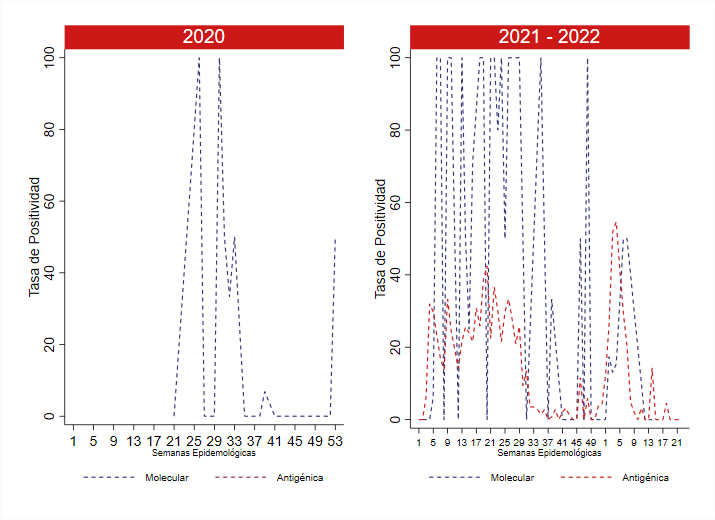
\includegraphics[width=0.7\linewidth]{../figuras/positividad_20_21_4}
			\end{center}
			{\footnotesize {Fuente de datos: NOTICOVID, SISCOVID.}}
		\end{figure}
		
		\begin{figure}[h]
			\caption{Exceso de Defunciones Comparativo en la Provincia de Canas 2020 y 2021, hasta la SE 43.}\label{fig:exceso_calca}
			\begin{center}
				\includegraphics[width=0.7\linewidth]{../figuras/exceso_4}
			\end{center}
			{\footnotesize {Fuente de datos: SINADEF.}}
		\end{figure}
		
		% Canas
		\clearpage
		
		\subsection*{Provincia de Canchis}
		\noindent Las figuras de abajo (Figura \ref{fig:inc_mort_canchis}, \ref{fig:positividad_canchis}) muestra que desde la SE 21 hubo un descenso de la Tasa de Mortalidad y Tasa de incidencia respecto a la semanas previas; sin embargo para la SE 41, la Tasa de Mortalidad tiene una pendiente en ascenso. En la Figura \ref{fig:exceso_canchis} se muestra que hay un exceso de 7 defunciones respecto al año 2020.
		
		\begin{figure}[h]
			\caption{Tasa de Incidencia y Mortalidad Comparativa en la Provincia de Canas 2020 y 2021, hasta la SE 43.}\label{fig:inc_mort_canchis}
			\begin{center}
				\includegraphics[width=0.7\linewidth]{../figuras/incidencia_mortalidad_20_21_5}
			\end{center}
			{\footnotesize {Fuente de datos: NOTICOVID, SISCOVID, SINADEF.}}
		\end{figure}
		
		\begin{figure}[h]
			\caption{Tasa de Positividad de Prueba Molecular y Antigénica Comparativa en la Provincia de Canas 2020 y 2021, hasta la SE 43.}\label{fig:positividad_canchis}
			\begin{center}
				\includegraphics[width=0.7\linewidth]{../figuras/positividad_20_21_5}
			\end{center}
			{\footnotesize {Fuente de datos: NOTICOVID, SISCOVID.}}
		\end{figure}
		
		\begin{figure}[h]
			\caption{Exceso de Defunciones Comparativo en la Provincia de Canas 2020 y 2021, hasta la SE 43.}\label{fig:exceso_canchis}
			\begin{center}
				\includegraphics[width=0.7\linewidth]{../figuras/exceso_5}
			\end{center}
			{\footnotesize {Fuente de datos: SINADEF.}}
		\end{figure}
		
		\clearpage
		
		% Chumbivilcas
		\subsection*{Provincia de Chumbivilcas}
		\noindent Las figuras de abajo (Figura \ref{fig:inc_mort_chumbivilcas}, \ref{fig:positividad_chumbivilcas}) muestra que desde la SE 21 hubo un descenso de la Tasa de Mortalidad y Tasa de incidencia respecto a la semanas previas; sin embargo para la SE 41, la Tasa de Mortalidad tiene una pendiente en ascenso. En la Figura \ref{fig:exceso_chumbivilcas} se muestra que hay un exceso de menos 1 defunciones respecto al año 2020.
		
		\begin{figure}[h]
			\caption{Tasa de Incidencia y Mortalidad Comparativa en la Provincia de Chumbivilcas 2020 y 2021, hasta la SE 43.}\label{fig:inc_mort_chumbivilcas}
			\begin{center}
				\includegraphics[width=0.7\linewidth]{../figuras/incidencia_mortalidad_20_21_6}
			\end{center}
			{\footnotesize {Fuente de datos: NOTICOVID, SISCOVID, SINADEF.}}
		\end{figure}
		
		\begin{figure}[h]
			\caption{Tasa de Positividad de Prueba Molecular y Antigénica Comparativa en la Provincia de Chumbivilcas 2020 y 2021, hasta la SE 43.}\label{fig:positividad_chumbivilcas}
			\begin{center}
				\includegraphics[width=0.7\linewidth]{../figuras/positividad_20_21_6}
			\end{center}
			{\footnotesize {Fuente de datos: NOTICOVID, SISCOVID.}}
		\end{figure}
		
		\begin{figure}[h]
			\caption{Exceso de Defunciones Comparativo en la Provincia de Chumbivilcas 2020 y 2021, hasta la SE 43.}\label{fig:exceso_chumbivilcas}
			\begin{center}
				\includegraphics[width=0.7\linewidth]{../figuras/exceso_6}
			\end{center}
			{\footnotesize {Fuente de datos: SINADEF.}}
		\end{figure}
		
		% Cusco
		\clearpage
		
		\subsection*{Provincia de Cusco}
		\noindent Las figuras de abajo (Figura \ref{fig:inc_mort_cusco}, \ref{fig:positividad_cusco}) muestra que desde la SE 21 hubo un descenso de la Tasa de Mortalidad y Tasa de incidencia respecto a la semanas previas; sin embargo para la SE 41 la Tasa de Incidencia mostró un pico de ascenso. En la Figura \ref{fig:exceso_cusco} se muestra que hay exceso de 2 defunciones respecto al año 2020.
		
		\begin{figure}[h]
			\caption{Tasa de Incidencia y Mortalidad Comparativa en la Provincia de Cusco 2020 y 2021, hasta la SE 43.}\label{fig:inc_mort_cusco}
			\begin{center}
				\includegraphics[width=0.7\linewidth]{../figuras/incidencia_mortalidad_20_21_7}
			\end{center}
			{\footnotesize {Fuente de datos: NOTICOVID, SISCOVID, SINADEF.}}
		\end{figure}
		
		\begin{figure}[h]
			\caption{Tasa de Positividad de Prueba Molecular y Antigénica Comparativa en la Provincia de Cusco 2020 y 2021, hasta la SE 43.}\label{fig:positividad_cusco}
			\begin{center}
				\includegraphics[width=0.7\linewidth]{../figuras/positividad_20_21_7}
			\end{center}
			{\footnotesize {Fuente de datos: NOTICOVID, SISCOVID.}}
		\end{figure}
		
		\begin{figure}[h]
			\caption{Exceso de Defunciones Comparativo en la Provincia de Cusco  2020 y 2021, hasta la SE 43.}\label{fig:exceso_cusco}
			\begin{center}
				\includegraphics[width=0.7\linewidth]{../figuras/exceso_7}
			\end{center}
			{\footnotesize {Fuente de datos: SINADEF.}}
		\end{figure}
		
		% Espinar
		\clearpage
		
		\subsection*{Provincia de Espinar}
		\noindent Las figuras de abajo (Figura \ref{fig:inc_mort_espinar}, \ref{fig:positividad_espinar}) muestra que desde la SE 25 la pendiente de la Tasa de Mortalidad e Incidencia ha ido en descenso respecto a las semanas previas. En la Figura \ref{fig:exceso_espinar} se muestra que hay exceso de 1 defunción respecto al año 2020.
		
		\begin{figure}[h]
			\caption{Tasa de Incidencia y Mortalidad Comparativa en la Provincia de Espinar 2020 y 2021, hasta la SE 43.}\label{fig:inc_mort_espinar}
			\begin{center}
				\includegraphics[width=0.7\linewidth]{../figuras/incidencia_mortalidad_20_21_8}
			\end{center}
			{\footnotesize {Fuente de datos: NOTICOVID, SISCOVID, SINADEF.}}
		\end{figure}
		
		\begin{figure}[h]
			\caption{Tasa de Positividad de Prueba Molecular y Antigénica Comparativa en la Provincia de Espinar 2020 y 2021, hasta la SE 43.}\label{fig:positividad_espinar}
			\begin{center}
				\includegraphics[width=0.7\linewidth]{../figuras/positividad_20_21_8}
			\end{center}
			{\footnotesize {Fuente de datos: NOTICOVID, SISCOVID.}}
		\end{figure}
		
		\begin{figure}[h]
			\caption{Exceso de Defunciones Comparativo en la Provincia de Espinar 2020 y 2021, hasta la SE 43.}\label{fig:exceso_espinar}
			\begin{center}
				\includegraphics[width=0.7\linewidth]{../figuras/exceso_8}
			\end{center}
			{\footnotesize {Fuente de datos: SINADEF.}}
		\end{figure}
		
		% La Convención
		\clearpage
		
		\subsection*{Provincia de La Convención}
		\noindent Las figuras de abajo (Figura \ref{fig:inc_mort_laconv}, \ref{fig:positividad_laconv}) muestra que desde la SE 25 la pendiente de la Tasa de Mortalidad e Incidencia ha ido en descenso respecto a las semanas previas con picos aislados entre semanas. En la Figura \ref{fig:exceso_laconv} se muestra que hay exceso de menos 9 defunciones respecto al año 2020.
		
		\begin{figure}[h]
			\caption{Tasa de Incidencia y Mortalidad Comparativa en la Provincia de La Convención 2020 y 2021, hasta la SE 43.}\label{fig:inc_mort_laconv}
			\begin{center}
				\includegraphics[width=0.7\linewidth]{../figuras/incidencia_mortalidad_20_21_9}
			\end{center}
			{\footnotesize {Fuente de datos: NOTICOVID, SISCOVID, SINADEF.}}
		\end{figure}
		
		\begin{figure}[h]
			\caption{Tasa de Positividad de Prueba Molecular y Antigénica Comparativa en la Provincia de La Convención 2020 y 2021, hasta la SE 43.}\label{fig:positividad_laconv}
			\begin{center}
				\includegraphics[width=0.7\linewidth]{../figuras/incidencia_mortalidad_20_21_9}
			\end{center}
			{\footnotesize {Fuente de datos: NOTICOVID, SISCOVID.}}
		\end{figure}
		
		\begin{figure}[h]
			\caption{Exceso de Defunciones Comparativo en la Provincia de La Convención 2020 y 2021, hasta la SE 43.}\label{fig:exceso_laconv}
			\begin{center}
				\includegraphics[width=0.7\linewidth]{../figuras/exceso_9}
			\end{center}
			{\footnotesize {Fuente de datos: SINADEF.}}
		\end{figure}
		
		% Paruro
		\clearpage
		
		\subsection*{Provincia de Paruro}
		\noindent Las figuras de abajo (Figura \ref{fig:inc_mort_paruro}, \ref{fig:positividad_paruro})  muestra que desde la SE 21 la Tasa de Mortalidad y Tasa muestran picos marcados entre semanas. Para la SE 41 la pendiente de la Tasa de Mortalidad se encuentra en ascenso. En la Figura \ref{fig:exceso_paruro} se muestra un exceso de 1 defunción respecto al año 2020.
		
		\begin{figure}[h]
			\caption{Tasa de Incidencia y Mortalidad Comparativa en la Provincia de Paruro 2020 y 2021, hasta la SE 43.}\label{fig:inc_mort_paruro}
			\begin{center}
				\includegraphics[width=0.7\linewidth]{../figuras/incidencia_mortalidad_20_21_10}
			\end{center}
			{\footnotesize {Fuente de datos: NOTICOVID, SISCOVID, SINADEF.}}
		\end{figure}
		
		\begin{figure}[h]
			\caption{Tasa de Positividad de Prueba Molecular y Antigénica Comparativa en la Provincia de Paruro 2020 y 2021, hasta la SE 43.}\label{fig:positividad_paruro}
			\begin{center}
				\includegraphics[width=0.7\linewidth]{../figuras/positividad_20_21_10}
			\end{center}
			{\footnotesize {Fuente de datos: NOTICOVID, SISCOVID.}}
		\end{figure}
		
		\begin{figure}[h]
			\caption{Exceso de Defunciones Comparativo en la Provincia de Paruro 2020 y 2021, hasta la SE 43.}\label{fig:exceso_paruro}
			\begin{center}
				\includegraphics[width=0.7\linewidth]{../figuras/exceso_10}
			\end{center}
			{\footnotesize {Fuente de datos: SINADEF.}}
		\end{figure}
		
		
		% Paucartambo
		\clearpage
		
		\subsection*{Provincia de Paucartambo}
		\noindent Las figuras de abajo (Figura \ref{fig:inc_mort_paucartam}, \ref{fig:positividad_paucartam}) muestra que desde la SE 25 la pendiente de la Tasa de Mortalidad e Incidencia ha ido en descenso respecto a las semanas previas con picos aislados entre semanas. En la Figura \ref{fig:exceso_paucartam} se muestra que no hay exceso de defunciones respecto al año 2020.
		
		\begin{figure}[h]
			\caption{Tasa de Incidencia y Mortalidad Comparativa en la Provincia de Paucartambo 2020 y 2021, hasta la SE 43.}\label{fig:inc_mort_paucartam}
			\begin{center}
				\includegraphics[width=0.7\linewidth]{../figuras/incidencia_mortalidad_20_21_11}
			\end{center}
			{\footnotesize {Fuente de datos: NOTICOVID, SISCOVID, SINADEF.}}
		\end{figure}
		
		\begin{figure}[h]
			\caption{Tasa de Positividad de Prueba Molecular y Antigénica Comparativa en la Provincia de Paucartambo 2020 y 2021, hasta la SE 43.}\label{fig:positividad_paucartam}
			\begin{center}
				\includegraphics[width=0.7\linewidth]{../figuras/positividad_20_21_11}
			\end{center}
			{\footnotesize {Fuente de datos: NOTICOVID, SISCOVID.}}
		\end{figure}
		
		\begin{figure}[h]
			\caption{Exceso de Defunciones Comparativo en la Provincia de Paucartambo 2020 y 2021, hasta la SE 43.}\label{fig:exceso_paucartam}
			\begin{center}
				\includegraphics[width=0.7\linewidth]{../figuras/exceso_11}
			\end{center}
			{\footnotesize {Fuente de datos: SINADEF.}}
		\end{figure}
		
		% Quispicanchi
		\clearpage
		
		\subsection*{Provincia de Quispicanchi}
		\noindent Las figuras de abajo (Figura \ref{fig:inc_mort_quisp}, \ref{fig:positividad_quisp}) muestra que desde la SE 25 la pendiente de la Tasa de Mortalidad e Incidencia ha ido en descenso respecto a las semanas previas con picos aislados entre semanas. En la Figura \ref{fig:exceso_quisp} se muestra que hay un exceso de menos 1 defunción respecto al año 2020.
		
		\begin{figure}[h]
			\caption{Tasa de Incidencia y Mortalidad Comparativa en la Provincia de Quispicanchi 2020 y 2021, hasta la SE 43.}\label{fig:inc_mort_quisp}
			\begin{center}
				\includegraphics[width=0.7\linewidth]{../figuras/incidencia_mortalidad_20_21_12}
			\end{center}
			{\footnotesize {Fuente de datos: NOTICOVID, SISCOVID, SINADEF.}}
		\end{figure}
		
		\begin{figure}[h]
			\caption{Tasa de Positividad de Prueba Molecular y Antigénica Comparativa en la Provincia de Quispicanchi 2020 y 2021, hasta la SE 43.}\label{fig:positividad_quisp}
			\begin{center}
				\includegraphics[width=0.7\linewidth]{../figuras/positividad_20_21_12}
			\end{center}
			{\footnotesize {Fuente de datos: NOTICOVID, SISCOVID.}}
		\end{figure}
		
		\begin{figure}[h]
			\caption{Exceso de Defunciones Comparativo en la Provincia de Quispicanchis 2020 y 2021, hasta la SE 43.}\label{fig:exceso_quisp}
			\begin{center}
				\includegraphics[width=0.7\linewidth]{../figuras/exceso_12}
			\end{center}
			{\footnotesize {Fuente de datos: SINADEF.}}
		\end{figure}
		
		% Urubamba
		\clearpage
		
		\subsection*{Provincia de Urubamba}
		\noindent Las figuras de abajo (Figura \ref{fig:inc_urub}, \ref{fig:positividad_urub}) muestra que desde la SE 25 la pendiente de la Tasa de Mortalidad e Incidencia ha ido en descenso respecto a las semanas previas con picos aislados entre semanas. En la Figura \ref{fig:exceso_urub} se muestra que hay exceso de menos 2 defunciones respecto al año 2020.
		
		\begin{figure}[h]
			\caption{Tasa de Incidencia y Mortalidad Comparativa en la Provincia de Urubamba 2020 y 2021, hasta la SE 43.}\label{fig:inc_urub}
			\begin{center}
				\includegraphics[width=0.7\linewidth]{../figuras/incidencia_mortalidad_20_21_13}
			\end{center}
			{\footnotesize {Fuente de datos: NOTICOVID, SISCOVID, SINADEF.}}
		\end{figure}
		
		\begin{figure}[h]
			\caption{Tasa de Positividad de Prueba Molecular y Antigénica Comparativa en la Provincia de Urubamba 2020 y 2021, hasta la SE 43.}\label{fig:positividad_urub}
			\begin{center}
				\includegraphics[width=0.7\linewidth]{../figuras/positividad_20_21_13}
			\end{center}
			{\footnotesize {Fuente de datos: NOTICOVID, SISCOVID.}}
		\end{figure}
		
		\begin{figure}[h]
			\caption{Exceso de Defunciones Comparativo en la Provincia de Urubamba 2020 y 2021, hasta la SE 43.}\label{fig:exceso_urub}
			\begin{center}
				\includegraphics[width=0.7\linewidth]{../figuras/exceso_13}
			\end{center}
			{\footnotesize {Fuente de datos: SINADEF.}}
		\end{figure}
		
		\clearpage
%---------------------------------------------------------------------------
		% CAPÍTULO: VARIANTES DE COVID-19
		%---------------------------------------------------------------------------
		%insertar el cover del capitulo
		\includepdf[pages={1}]{../editorial/6.pdf}
		\clearpage
		
		\section* {Variantes de COVID-19 en la Región Cusco}
		\addcontentsline{toc}{chapter}{Variantes de COVID-19}
		\noindent La preocupación por las variantes de SARS CoV-2 se ha incrementado en el tiempo, en la Figura \ref{fig:variantes} se muestra la evolución del tipo de variantes aisladas en nuestra región. Para el mes de Noviembre se realizó secuenciamiento genético a 13 muestras positivas por COVID-19, de las cuáles el 92$\%$ fueron genotipificadas como variante Delta y el 8$\%$ restante como variante Gamma.
		
			
		\begin{figure}[h]
			\caption{Prevalencia de las variantes de SARS Cov2 aisladas en la región de Cusco, hasta la SE 43. }\label{fig:variantes}
			\begin{center}
				\includegraphics[width=0.85\linewidth]{../figuras/variantes.pdf}
			\end{center}
			{\footnotesize {Fuente de datos: INS-NETLAB, UPCH, UNSAAC}}
		\end{figure}
	
	
	Asímismo, la Figura \ref{fig:mapa_variantes}  muestra el lugar de aislamiento de las Variantes encontradas en la Región. Se presenta el número de casos acumulados, la Variante Lamba tiene el mayor número de casos acumulados sobretodo provincia de Cusco y Quispicanchis, seguida de la Variante Delta, con la mayoría de casos aislados en la Provincia Cusco. 
	
	
  
			\begin{figure}[h]
				\caption{Distribución provincial de las variantes de SARS-Cov-2 aisladas en la Región Cusco, hasta la SE 47.}
				\label{fig:mapa_variantes}
				\centering
				\begin{subfigure}[b]{0.40\textwidth}
					\centering
					\includegraphics[width=\textwidth]{../figuras/variantes_provincial_lambda.pdf}
					\caption{Variante Lambda}
					%\label{fig:}
				\end{subfigure}
				\hfill
				\begin{subfigure}[b]{0.40\textwidth}
					\centering
					\includegraphics[width=\textwidth]{../figuras/variantes_provincial_gamma.pdf}
					\caption{Variante Gamma}
					%\label{fig:70 a 79 años}
				\end{subfigure}
				
				\vspace{10mm}
				\begin{subfigure}[b]{0.40\textwidth}
					\centering
					\includegraphics[width=\textwidth]{../figuras/variantes_provincial_delta.pdf}
					\caption{Variante Delta}
					%\label{fig:60 a 69 años}
				\end{subfigure}
			\end{figure}

\clearpage
%---------------------------------------------------------------------------
% CAPÍTULO: DEFUNCIONES CERO
%-------------------------------------------

%insertar el cover del capitulo
\includepdf[pages={1}]{../editorial/7.pdf}
\clearpage
	\section*{Semanas con Cero Defunciones por COVID-19 por Semana a Nivel Provincial}\addcontentsline{toc}{chapter}{Defunciones Cero}
	
	\noindent En la tabla inferior se muestra las provincias con Cero defunciones reportadas (casillas en amarillo) por cada semana epidemiológica. Se evidencia que para la SE 43, 10 de las 13 provincias de la Región Cusco no reportaron muertes en su territorio.Notablemente, las provincias de Acomayo, Calca, Espinar, Paucartambo han tenido \textbf{\color{mycolor2}una} defunción por COVID-19 en las últimas 9 semanas epidemológicas. La última semana (SE43) sólo se registraron defunciones en Chumbivilcas Cusco, y Paruro.
	
	\begin{table}[h]
		\resizebox{\textwidth}{!}{%
			\begin{tabular}{lccccccccc}
	\textbf{}              	  
	& \multicolumn{1}{l}{}                        
	& \multicolumn{1}{l}{}      
	& \multicolumn{1}{l}{}                         
	& \multicolumn{1}{l}{}                         
	& \multicolumn{1}{l}{}                         
	& \multicolumn{1}{l}{}                        
	& \multicolumn{1}{l}{}                         
	& \multicolumn{1}{l}{} \\                   
	\textbf{}                                                                 				
	&\textbf{SE-31} 							
	&\textbf{SE-32}						
	&\textbf{SE-33}								
	&\textbf{SE-34}					
	&\textbf{SE-35}								
	&\textbf{SE-36}
	&\textbf{SE-37}
	&\textbf{SE-38}\\							
	\textbf{}              	  																
	&\textbf{31jul-06ago}						
	&\textbf{07ago-13ago}						
	&\textbf{14ago-20ago}						
	&\textbf{21ago-27ago}						
	&\textbf{28ago-03sep}
	&\textbf{04sep-10sep}
	&\textbf{11sep-17sep} 
	&\textbf{18sep-24sep} \\
	\textbf{Acomayo}                        												
	&\cellcolor[HTML]{FCC46C}
	&\cellcolor[HTML]{FCC46C}					
	&\cellcolor[HTML]{FCC46C}
	&\cellcolor[HTML]{FCC46C}					
	&\cellcolor[HTML]{FCC46C}
	&\cellcolor[HTML]{FCC46C} 
	&\cellcolor[HTML]{FCC46C}
	&\cellcolor[HTML]{FCC46C}\\
	\textbf{Anta}                                                  				
	&1											
	&\cellcolor[HTML]{FCC46C}					
	&\cellcolor[HTML]{FCC46C}					
	&\cellcolor[HTML]{FCC46C}					
	&\cellcolor[HTML]{FCC46C}
	&\cellcolor[HTML]{FCC46C}	
	&\cellcolor[HTML]{FCC46C}
	&\cellcolor[HTML]{FCC46C}\\					
	\textbf{Calca}      				       									
	&\cellcolor[HTML]{FCC46C}					
	&1											
	&\cellcolor[HTML]{FCC46C}					
	&1											
	&\cellcolor[HTML]{FCC46C}
	&1
	&1
	&\cellcolor[HTML]{FCC46C}\\          			
	\textbf{Canas}                              									
	&\cellcolor[HTML]{FCC46C}
	&1											
	&1
	&\cellcolor[HTML]{FCC46C}					
	&\cellcolor[HTML]{FCC46C}
	&\cellcolor[HTML]{FCC46C}	
	&\cellcolor[HTML]{FCC46C}
	&\cellcolor[HTML]{FCC46C}\\	
	\textbf{Canchis}    						
	&1			
	&\cellcolor[HTML]{FCC46C}					
	&\cellcolor[HTML]{FCC46C}			
	&\cellcolor[HTML]{FCC46C}					
	&1
	&1
	&\cellcolor[HTML]{FCC46C}
	&\cellcolor[HTML]{FCC46C}\\											
	\textbf{Chumbivilcas}                      									
	&\cellcolor[HTML]{FCC46C}
	&\cellcolor[HTML]{FCC46C}					
	&\cellcolor[HTML]{FCC46C}
	&\cellcolor[HTML]{FCC46C}					
	&1
	&\cellcolor[HTML]{FCC46C}
	&1
	&1\\
	\textbf{Cusco}      															
	&2		
	&3											
	&2
	&4											
	&1
	&1
	&\cellcolor[HTML]{FCC46C}
	&\cellcolor[HTML]{FCC46C}\\								
	\textbf{Espinar}       					             							
	&\cellcolor[HTML]{FCC46C}					
	&\cellcolor[HTML]{FCC46C}
	&\cellcolor[HTML]{FCC46C}					
	&\cellcolor[HTML]{FCC46C}
	&\cellcolor[HTML]{FCC46C}					
	&\cellcolor[HTML]{FCC46C}
	&\cellcolor[HTML]{FCC46C}
	&\cellcolor[HTML]{FCC46C}\\	
	\textbf{La Convención}       
	&3											
	&1											
	&2											
	&1											
	&3
	&\cellcolor[HTML]{FCC46C}
	&\cellcolor[HTML]{FCC46C}
	&\cellcolor[HTML]{FCC46C}\\	
	\textbf{Paruro}                            					
	&\cellcolor[HTML]{FCC46C}					
	&\cellcolor[HTML]{FCC46C}					
	&\cellcolor[HTML]{FCC46C}					
	&\cellcolor[HTML]{FCC46C}					
	&\cellcolor[HTML]{FCC46C}
	&\cellcolor[HTML]{FCC46C} 					
	&\cellcolor[HTML]{FCC46C}
	&\cellcolor[HTML]{FCC46C}\\
	\textbf{Paucartambo}               		                       					
	&\cellcolor[HTML]{FCC46C}					
	&\cellcolor[HTML]{FCC46C}
	&\cellcolor[HTML]{FCC46C}					
	&\cellcolor[HTML]{FCC46C}
	&\cellcolor[HTML]{FCC46C}					
	&\cellcolor[HTML]{FCC46C}
	&\cellcolor[HTML]{FCC46C}
	&\cellcolor[HTML]{FCC46C}\\
	\textbf{Quispicanchi}          	      				
	&1											
	&\cellcolor[HTML]{FCC46C}					
	&1											
	&\cellcolor[HTML]{FCC46C}					
	&1
	&\cellcolor[HTML]{FCC46C}
	&\cellcolor[HTML]{FCC46C}
	&\cellcolor[HTML]{FCC46C}\\
	\textbf{Urubamba}  					
	&1											
	&\cellcolor[HTML]{FCC46C}					
	&\cellcolor[HTML]{FCC46C}					
	&1											
	&1	
	&\cellcolor[HTML]{FCC46C}
	&\cellcolor[HTML]{FCC46C}
	&\cellcolor[HTML]{FCC46C}\\						
	&\multicolumn{1}{l}{}                       &\multicolumn{1}{l}{}            &\multicolumn{1}{l}{}                         
	&\multicolumn{1}{l}{}                       &\multicolumn{1}{l}{}            &\multicolumn{1}{l}{}                       &\multicolumn{1}{l}{}                       &\multicolumn{1}{l}{}            			    
\end{tabular}
		}
		{\footnotesize {Fuente de datos: SINADEF.}}
	\end{table}
\pagebreak

%---------------------------------------------------------------------------
% CAPÍTULO: AGRADECIMIENTOS
%---------------------------------------------------------------------------
	\section*{Agradecimientos}
	\addcontentsline{toc}{chapter}{Agradecimientos}
		
	\centering
		{\large El presente Boletín Epidemiológico COVID-19 se ha elaborado gracias a la información y esfuerzo conjunto de los Equipos de Inteligencia Sanitaria de los Hospitales y Redes de la GERESA Cusco:

		\vspace{0.5cm}
		\noindent
		\begin{minipage}[t]{.45\textwidth}
			\centering
			Hospital Regional del Cusco \\
			M.S.P. Marina Ochoa Linares \vspace{0.5cm}\\
			Hospital Antonio Lorena \\
			Dr. Homero Dueñas \vspace{.5cm}\\
			Hospital Nacional Adolfo Guevara Velazco\\
			M.S.P. Lucio Velasquez Cuentas \vspace{.5cm}\\
			Red de Salud Norte \\
			M.C. Guido Giraldo Alencastre\vspace{0.5cm}\\
			Red de Salud Sur\\
			Lic. Luz Marina Bernable Villasante \vspace{0.5cm}\\	
		\end{minipage}
		\hfill
		\noindent
		\begin{minipage}[t]{.45\textwidth}
			\centering
			Red de Salud La Convención\\
			Dr. David Coanqui Pacori\vspace{0.5cm}\\
			Red de Salud Chumbivilcas\\
			Lic. Eduarda Benito Calderón \vspace{.5cm}\\
			Red de Salud Canas Canchis Espinar\\
			MC. William Achahui Mercado \vspace{.5cm}\\
			Red de Salud Kimbiri Pichari \\
			Lic Fiorela Alvarez Nihua\vspace{0.5cm}\\	
		\end{minipage}
%---------------------------------------------------------------------------
% CAPÍTULO: AGRADECIMIENTOS
%---------------------------------------------------------------------------
	\chapter*{Diseño y Edición}
	\addcontentsline{toc}{chapter}{Diseño y Edición}
	\begin{center}
	
	% Como siempre, por orden alfabético del apellid0
	
	MSC. Fátima R. Concha Velasco
	
	M.C. Ana Gabriela Eulalia Moncada Arias 
	
	Ing. Joel Wilfredo Sumerente Ayerbe
	\end{center}

	%insertar la última página
	\includepdf[pages={1}]{../editorial/pagina_final.pdf}
	\clearpage
	
\end{document}